% Options for packages loaded elsewhere
\PassOptionsToPackage{unicode}{hyperref}
\PassOptionsToPackage{hyphens}{url}
\PassOptionsToPackage{dvipsnames,svgnames,x11names}{xcolor}
%
\documentclass[
  11pt,
  letterpaper,
]{article}

\usepackage{amsmath,amssymb}
\usepackage{iftex}
\ifPDFTeX
  \usepackage[T1]{fontenc}
  \usepackage[utf8]{inputenc}
  \usepackage{textcomp} % provide euro and other symbols
\else % if luatex or xetex
  \usepackage{unicode-math}
  \defaultfontfeatures{Scale=MatchLowercase}
  \defaultfontfeatures[\rmfamily]{Ligatures=TeX,Scale=1}
\fi
\usepackage{lmodern}
\ifPDFTeX\else  
    % xetex/luatex font selection
\fi
% Use upquote if available, for straight quotes in verbatim environments
\IfFileExists{upquote.sty}{\usepackage{upquote}}{}
\IfFileExists{microtype.sty}{% use microtype if available
  \usepackage[]{microtype}
  \UseMicrotypeSet[protrusion]{basicmath} % disable protrusion for tt fonts
}{}
\makeatletter
\@ifundefined{KOMAClassName}{% if non-KOMA class
  \IfFileExists{parskip.sty}{%
    \usepackage{parskip}
  }{% else
    \setlength{\parindent}{0pt}
    \setlength{\parskip}{6pt plus 2pt minus 1pt}}
}{% if KOMA class
  \KOMAoptions{parskip=half}}
\makeatother
\usepackage{xcolor}
\usepackage[margin=1in]{geometry}
\setlength{\emergencystretch}{3em} % prevent overfull lines
\setcounter{secnumdepth}{5}
% Make \paragraph and \subparagraph free-standing
\ifx\paragraph\undefined\else
  \let\oldparagraph\paragraph
  \renewcommand{\paragraph}[1]{\oldparagraph{#1}\mbox{}}
\fi
\ifx\subparagraph\undefined\else
  \let\oldsubparagraph\subparagraph
  \renewcommand{\subparagraph}[1]{\oldsubparagraph{#1}\mbox{}}
\fi


\providecommand{\tightlist}{%
  \setlength{\itemsep}{0pt}\setlength{\parskip}{0pt}}\usepackage{longtable,booktabs,array}
\usepackage{calc} % for calculating minipage widths
% Correct order of tables after \paragraph or \subparagraph
\usepackage{etoolbox}
\makeatletter
\patchcmd\longtable{\par}{\if@noskipsec\mbox{}\fi\par}{}{}
\makeatother
% Allow footnotes in longtable head/foot
\IfFileExists{footnotehyper.sty}{\usepackage{footnotehyper}}{\usepackage{footnote}}
\makesavenoteenv{longtable}
\usepackage{graphicx}
\makeatletter
\def\maxwidth{\ifdim\Gin@nat@width>\linewidth\linewidth\else\Gin@nat@width\fi}
\def\maxheight{\ifdim\Gin@nat@height>\textheight\textheight\else\Gin@nat@height\fi}
\makeatother
% Scale images if necessary, so that they will not overflow the page
% margins by default, and it is still possible to overwrite the defaults
% using explicit options in \includegraphics[width, height, ...]{}
\setkeys{Gin}{width=\maxwidth,height=\maxheight,keepaspectratio}
% Set default figure placement to htbp
\makeatletter
\def\fps@figure{htbp}
\makeatother
\newlength{\cslhangindent}
\setlength{\cslhangindent}{1.5em}
\newlength{\csllabelwidth}
\setlength{\csllabelwidth}{3em}
\newlength{\cslentryspacingunit} % times entry-spacing
\setlength{\cslentryspacingunit}{\parskip}
\newenvironment{CSLReferences}[2] % #1 hanging-ident, #2 entry spacing
 {% don't indent paragraphs
  \setlength{\parindent}{0pt}
  % turn on hanging indent if param 1 is 1
  \ifodd #1
  \let\oldpar\par
  \def\par{\hangindent=\cslhangindent\oldpar}
  \fi
  % set entry spacing
  \setlength{\parskip}{#2\cslentryspacingunit}
 }%
 {}
\usepackage{calc}
\newcommand{\CSLBlock}[1]{#1\hfill\break}
\newcommand{\CSLLeftMargin}[1]{\parbox[t]{\csllabelwidth}{#1}}
\newcommand{\CSLRightInline}[1]{\parbox[t]{\linewidth - \csllabelwidth}{#1}\break}
\newcommand{\CSLIndent}[1]{\hspace{\cslhangindent}#1}

\usepackage{amsfonts}
\DeclareMathAlphabet{\mathams}{U}{msb}{m}{n}
\usepackage{algorithm}
\usepackage{algpseudocode}
\usepackage{setspace}
\doublespacing
\makeatletter
\makeatother
\makeatletter
\makeatother
\makeatletter
\@ifpackageloaded{caption}{}{\usepackage{caption}}
\AtBeginDocument{%
\ifdefined\contentsname
  \renewcommand*\contentsname{Table of contents}
\else
  \newcommand\contentsname{Table of contents}
\fi
\ifdefined\listfigurename
  \renewcommand*\listfigurename{List of Figures}
\else
  \newcommand\listfigurename{List of Figures}
\fi
\ifdefined\listtablename
  \renewcommand*\listtablename{List of Tables}
\else
  \newcommand\listtablename{List of Tables}
\fi
\ifdefined\figurename
  \renewcommand*\figurename{Figure}
\else
  \newcommand\figurename{Figure}
\fi
\ifdefined\tablename
  \renewcommand*\tablename{Table}
\else
  \newcommand\tablename{Table}
\fi
}
\@ifpackageloaded{float}{}{\usepackage{float}}
\floatstyle{ruled}
\@ifundefined{c@chapter}{\newfloat{codelisting}{h}{lop}}{\newfloat{codelisting}{h}{lop}[chapter]}
\floatname{codelisting}{Listing}
\newcommand*\listoflistings{\listof{codelisting}{List of Listings}}
\makeatother
\makeatletter
\@ifpackageloaded{caption}{}{\usepackage{caption}}
\@ifpackageloaded{subcaption}{}{\usepackage{subcaption}}
\makeatother
\makeatletter
\@ifpackageloaded{tcolorbox}{}{\usepackage[skins,breakable]{tcolorbox}}
\makeatother
\makeatletter
\@ifundefined{shadecolor}{\definecolor{shadecolor}{rgb}{.97, .97, .97}}
\makeatother
\makeatletter
\makeatother
\makeatletter
\makeatother
\ifLuaTeX
  \usepackage{selnolig}  % disable illegal ligatures
\fi
\IfFileExists{bookmark.sty}{\usepackage{bookmark}}{\usepackage{hyperref}}
\IfFileExists{xurl.sty}{\usepackage{xurl}}{} % add URL line breaks if available
\urlstyle{same} % disable monospaced font for URLs
\hypersetup{
  pdftitle={A Review of Methods for Explainable and Interpretable Graph Neural Networks},
  pdfauthor={Art Tay},
  colorlinks=true,
  linkcolor={blue},
  filecolor={Maroon},
  citecolor={Blue},
  urlcolor={Blue},
  pdfcreator={LaTeX via pandoc}}

\title{A Review of Methods for Explainable and Interpretable Graph
Neural Networks}
\author{Art Tay}
\date{}

\begin{document}
\maketitle
\ifdefined\Shaded\renewenvironment{Shaded}{\begin{tcolorbox}[breakable, enhanced, borderline west={3pt}{0pt}{shadecolor}, boxrule=0pt, sharp corners, frame hidden, interior hidden]}{\end{tcolorbox}}\fi

\hypertarget{introduction}{%
\section{Introduction}\label{introduction}}

\quad Graphs provide an incredibly flexible structure for modeling
complex data. Data can naturally appear as graphs, like molecules. We
can reduce data to a graph, such as the key points of a image. We can
even use graphs to add structure, such as grammatical relationships.
Graph Neural Networks (GNNs) have become a popular choice for prediction
and inference on graph data. At their core, GNNs work by iteratively
updating node embeddings based on information from neighboring nodes.
The idea is to use the graph's structure to engineer better features.
This message passing scheme allows GNNs to capture complex dependencies
and patterns present within the graph structure. GNN architectures
typically consist of multiple layers, each performing message passing
and aggregation operations to refine the embeddings. These layers are
often followed by pooling and dense prediction layers to produce the
final output. Some important applications of graph classification
include predicting chemical toxicity
(\protect\hyperlink{ref-bai2019unsupervised}{Bai et al. 2019}),
classifying proteins
(\protect\hyperlink{ref-gallicchio2019fast}{Gallicchio and Micheli
2019}), and even detecting cancer from pathology slides
(\protect\hyperlink{ref-Xiao_Wang_Rong_Yang_Zhang_Zhan_Bishop_Wilhelm_Zhang_Pickering_et_al._2023}{Xiao
et al. 2023}). While GNNs achieve remarkable predictive power, their
complexity prevents the exaction of the scientific rationale. Like many
deep learning models, the black box nature of GNNs prevents wide
adoption. Without strong methods for understanding their predictions,
GNNs are more susceptible to adversarial attacks and undetected
discrimination. Inferential methods also serve to direct modeling
efforts by highlighting common structures or features that may be
predictive in other applications. These reasons underscore the critical
importance of methods for explaining and interpreting GNN models.

\quad Although explainability and interpretability are sometimes used
interchangeably in the literature, we will adopt the distinction
expressed in Yuan et al.
(\protect\hyperlink{ref-Yuan_Yu_Gui_Ji_2022}{2022}). In this article the
authors say that a model is explainable if the models predictions can be
reasoned post-hoc (\protect\hyperlink{ref-Yuan_Yu_Gui_Ji_2022}{Yuan et
al. 2022}). For example, the effect of a specific input variable can be
estimated by either dropping or randomly permuting the variable and
accessing the effect on the output
(\protect\hyperlink{ref-Breiman_2001}{Breiman 2001}). This paradigm
could be directly applied to GNNs; however, researchers are often not
interested in the statistical significance of tabular node and
edge-level features. Most scientific questions focus on the importance
of specific graph-level substructures. The challenge with GNN
explanations is that, in addition to computing the importance of
features, the high-level features themselves must first be identified.
On the other hand, a model is interpretable if the model's decision
process can be readily understood by humans
(\protect\hyperlink{ref-Yuan_Yu_Gui_Ji_2022}{Yuan et al. 2022}). For
example, a linear regression model is interpretable because each
coefficient clearly defines the relationship between any input and
output. An interpretable model is typically superior to an explainable
one because similar to a partial F-test, explanation methods might
identify that certain variables enhance the model, but they cannot
explain how these variables contribute. On the flip side, interpretable
models may not reach the performance levels of black-box models. GNN
models are generally not interpretable because the relation expressed by
the parameters tends to exceed human understanding. A direct translation
from traditional statistics would be a circuit type analysis, which has
work for image processing convolution neural networks
(\protect\hyperlink{ref-olah2020zoom}{Olah et al. 2020}). For graphs,
this would involve using coefficients on subgraphs to produce
predictions. Similar to the difficulties of explanation methods, these
subgraphs would have to be identified, which can be computational
complex and expensive given the combinatorial nature of graphs.
Overcoming these challenges has substantial scientific impacts. In
applications where GNNs demonstrate strong predictive power, it enables
the formulation of testable scientific hypotheses about the nature of
the classification. Conversely, in cases where GNNs exhibit weak
predictive power, it helps identify and understand potential
misunderstandings within the model.

\hypertarget{general-notation}{%
\subsection{General Notation}\label{general-notation}}

\begin{itemize}
\item
  Any graph \(G\) can be describe by \(X, A, E\). The node feature,
  matrix, edge feature matrix, and adjacency matrix respectively.
\item
  Let \(X = [X_c, \ X_d]\), where \(X_c\) is the subset of continuous
  node features and \(X_d\) is the subset of one-hot discrete node
  features.
\item
  Let \(E = [E_c, \ E_d]\), denoted in the same manner.
\item
  Let \(n\) represent the number of nodes in the graph and \(v\)
  represent the number of edges.
\item
  For any graph, let \(\nu\) denote the set of node and \(\mathcal{E}\)
  denote the set of edges.
\item
  Let \(\text{feat}_{(.)}\) denote the number of features or columns in
  the the corresponding feature matrix.
\item
  \(A\) is a binary \(n \times n\) matrix where \(A[i, \ j] = 1\)
  indicates that an edge exists between nodes labeled \(i\) and \(j\).
\item
  Let
  \(\text{explainee}(G; \ \Omega) = h^{(1)}_G, \dots h^{(L)}_G, \rho_G\)
  be an \(L\) layer GNN model with parameters \(\Omega\) that we would
  like to explain.
\item
  Let \(\hat Y_G\) be the predicted class label for graph \(G\)
  predicted from explainee().
\item
  Unless otherwise noted, assume any GNN model discussed is a
  graph-level classification model.
\end{itemize}

\hypertarget{analysis-of-core-papers}{%
\section{Analysis of Core Papers}\label{analysis-of-core-papers}}

\hypertarget{gnninterpreter-wang_shen_2024}{%
\subsection{\texorpdfstring{GNNInterpreter
(\protect\hyperlink{ref-Wang_Shen_2024}{X. Wang and Shen
2024})}{GNNInterpreter (X. Wang and Shen 2024)}}\label{gnninterpreter-wang_shen_2024}}

\quad GNNInterpreter (\protect\hyperlink{ref-Wang_Shen_2024}{X. Wang and
Shen 2024}) is a method for generating model-level explanations of GNN
graph classification models. In general, explanation methods serve to
elucidate which features within the data influence disparate
predictions. These methods typically fall into two categories:
instance-level and model-level. Instance-level explanations aim to
unveil the model's rationale behind a particular prediction. In domains
such as image and text analysis, a prevalent approach involves masking
or perturbing the instance and assessing the impact on the model's
prediction. On the other hand, model-level explanations seek to
understand how a model generally distinguishes between classes. In image
and text analysis, for instance, one common technique involves treating
the input as a trainable parameter and optimizing the model's prediction
towards a specific class. Consequently, the resulting optimized input
comprises a set of features strongly associated with the targeted class.
GNNInterpreter provides model level explanations for GNN in this manner.
Formally, GNNInterpreter tries to learn the graph generating
distribution for each class. GNNInterpreter works by optimizing the
parameters of a generic graph generating distribution to produce samples
that closely match the explainee's understanding of the targeted class.

\quad Graph generating distributions are hard to specify because there
can be discrete and continuous elements of \(X\), \(E\) and \(A\).
Furthermore, the interactions between these matrices can be complex. The
authors tackle these issues by making two simplify assumptions. First,
they assume that every graph is a \emph{Gilbert random graph}
(\protect\hyperlink{ref-Gilbert_1959}{Gilbert 1959}), where every
possible edge as an independent fixed probability of occurring. Second,
the author assume that the features of every node and edge are
independently distributed. The justification of the first assumption is
that the other common types of random graphs are not suitable for this
application. Erdo-Renyi random graphs
(\protect\hyperlink{ref-erdds1959random}{ERDdS and R\&wi 1959}) have a
fixed number of edges, which limits the diversity of explanations, Rado
random graphs (\protect\hyperlink{ref-Rado1964UniversalGA}{Rado 1964})
are infinite in size, and the random dot-product graph model is just a
generalization of Gilbert's model. The second assumption is justified by
the fact that the parameters of the independent distributions will be
updated jointly using the \emph{explainee} model. Therefore, the
\emph{explainee's} understanding of the latent correlation structure
should be contained in the final estimates.

\quad Although the graphs discuss in this paper only contain discrete
features, \(X_c\) and \(E_c\) can be sampled from any continuous
distribution that can be expressed as a location-scale family.
Separating the stochastic and systematic components is necessary for
gradient based optimization. It is commonly known as the
\emph{reparametrization trick}. The discrete feature matrices, (\(X_d\),
\(E_d\), \(A\)), need to be sampled from a continuous distribution for
gradient based optimization, but the distribution has to have sampling
properties close to a discrete distribution. The author assume that the
true underlying distribution for every discrete node and edge feature is
\emph{categorical}. The categorical distribution is also know as the
multi-bernoulli, where every sample has a fixed probability of being in
one of the discrete categories. Let \(\theta_\text{cat}\) represent the
associated vector of un-normalized or relative probabilities, where each
entries is \(>0\). Then,

\begin{equation} \label{gumbel-max-eq}
    \text{argmax} \ \log \theta_\text{cat} + \text{Gumbel}(0, 1)
        \sim \text{Cat}(\theta_\text{cat})
\end{equation}

The intuition is that the Gumbel distribution, which is the density of
the maximum order statistic of i.i.d. standard normals, makes it a good
candidate for modeling the winning or maximum probability category.
Adding Gumbel noise to the logits should maintain the true relative
proportions, but enough skewness such that every category has some
probability of having the maximum noised logit. A proof of equation
\ref{gumbel-max-eq} is provide in section Section~\ref{sec-proof}.
Approximating the argmax function with the Softmax function allows for
approximate categorical sampling that is differentiable w.r.t.
\(\theta_\text{cat}\). The associate inverse uniform CDF sampling
formula below is referred to as the \emph{Gumbel-Softmax trick} or the
\emph{concrete distribution}
(\protect\hyperlink{ref-Maddison_Mnih_Teh_2017}{Maddison, Mnih, and Teh
2017}). \begin{equation}
    \text{Softmax}
    \left(
        \dfrac{\log \theta_{\text{Cat}} - log(-log \ \epsilon)}{\tau}
    \right), \quad \epsilon \sim U[0, 1].
\end{equation} \(\tau\) is a hyperparameter that controls the degree of
relaxation. Smaller value of \(\tau\) approximate the discrete sampling
better, but can result in numerical issues. The adjacency matrix can be
sampled in a similar manner since the Bernoulli is just a special case
of the categorical.\\
\begin{equation} \label{binary-concrete}
        \text{sigmoid}
            \left(\dfrac{\log(\theta_A / (1 - \theta_A)) + \log \ \epsilon - \log(1 - \log \ \epsilon)}{\tau} \right), \quad \epsilon \sim U[0, 1], 
    \end{equation} where \(\theta_A\) is an \(n \times n\) matrix with
each \([i, j]\) entry representing the relative probability that the
\(ij\) edge exists. Equation \ref{binary-concrete} samples from the
\emph{binary concrete distribution}
(\protect\hyperlink{ref-Maddison_Mnih_Teh_2017}{Maddison, Mnih, and Teh
2017}). Taken together, let\\
\[
    G_{\text{gen}} \sim \text{gen}(\Theta)  
\]

notate the combined graph generating distribution, where \(\Theta\) is
the set of all parameters from the independently sampled distributions.

\quad An obvious objective is to maximize the likelihood that the
\emph{explainee} model predicts a sampled graph to be a member of the
target class. Let \(\tilde{\rho}\) denote the desired predicted
probability vector. Then the above objective can be expressed as:
\begin{equation} \label{l-pred}
        \mathcal{L}_\text{pred} (\Theta \ | \ G_\text{gen}) = \mathams{E}_{G_\text{gen}} \ \text{CrsEnt} (\text{explainee}(G_\text{gen}), \ \tilde{\rho})
    \end{equation} While the above objective enforces a desirable
property, it fails to be restrictive enough to generate realistic
graphs. This is because the final prediction, \(\rho_{G_{\text{gen}}}\)
is compute using only final embeddings, \(h^{(L)}_{G_{\text{gen}}}\).
Normally \(h^{(L)}_{G_{\text{gen}}}\) contains all the needed
information from the graphs structure; however, the generation scheme
allows the feature distribution to be optimized directly. This means
that an explanation can ignore the graph structure and optimize towards
the desired final embeddings. It is dangerously common for nonsensical
features and structures at the graph level to end up on the desired side
of the decision boundary. Empirically, the authors found that even
completely random graphs can produce confidence and consistent
predictions.

\begin{figure}

{\centering 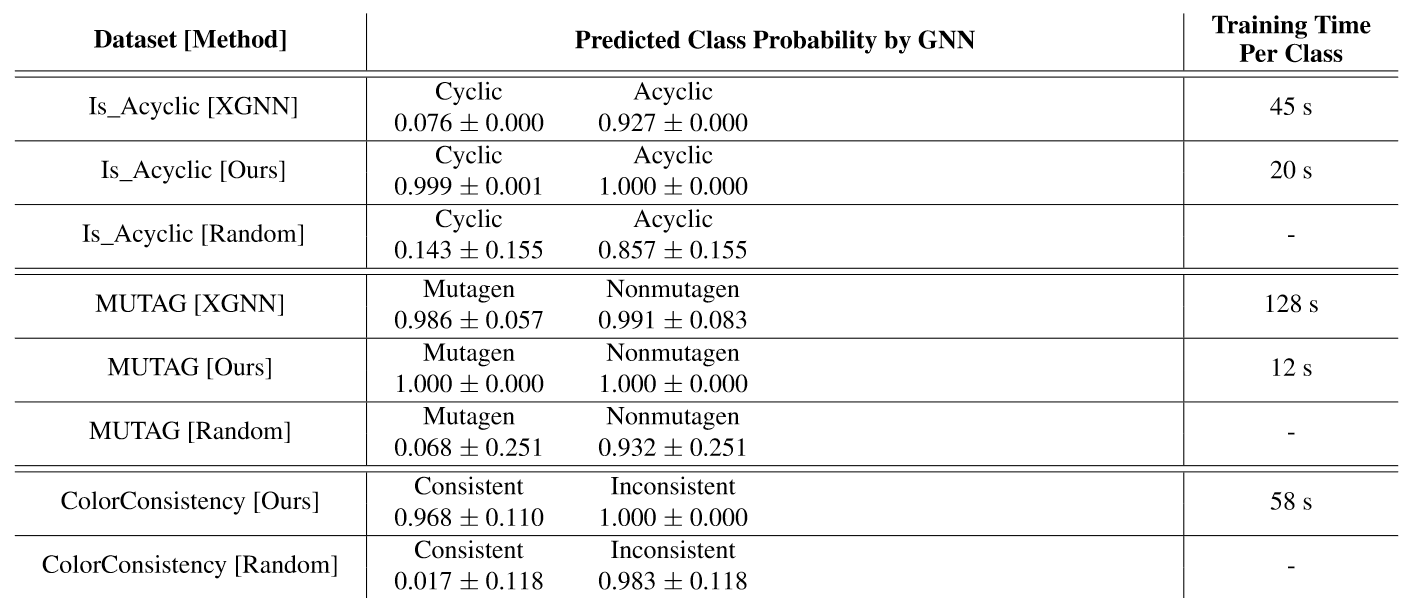
\includegraphics[width=0.9\textwidth,height=\textheight]{figures/random_baseline.png}

}

\caption{\label{fig-random-baseline}An abridged copy of Table 5 from X.
Wang and Shen (\protect\hyperlink{ref-Wang_Shen_2024}{2024}).}

\end{figure}

For example, Figure~\ref{fig-random-baseline} shows that random graphs
had an average predicted probability of being non-mutagenic in the MUTAG
dataset (\protect\hyperlink{ref-Debnath_1991}{Debnath et al. 1991}) if
93.2\%. In order to mitigate this issue, the authors proposed additional
minimizing the cosine distance between the average embedding of all the
observed graph from the targeted class, \(\bar h^{(L)}_{G_c}\), and the
embedding of the generated explanation: \begin{equation} \label{l-embed}
       \mathcal{L}_{\text{embed}}(\Theta \ | \ G_\text{gen}) = 
            \mathams{E}_{G_\text{gen}}
            \text{CosDist}\left( \bar h^{(L)}_{G_c}, \ h^{(L)}_{G_\text{gen}} \right). 
    \end{equation}

Additionally, the author wanted to encourage sparsity for ease of
interpretation. This was done by employing an \(L_1\), \(L_2\), and a
budget penalty on the edge probabilities:\\
\begin{equation} \label{l-spars}
        \mathcal{L}_{\text{spars}}(\theta_A) = ||\theta_A||_1 + ||\theta_A||_2 + \text{softplus}(\text{sigmoid}||\theta_A||_1 - B)^2, 
    \end{equation} where \(B\) is the expected maximum number of edge
for generated explanation graphs.Connectivity is another desirable
property as it ensures a cohesive explanation. To encourage connectivity
the author minimize the \emph{KL-Divergence} between edge probabilities
that share a common node. \begin{equation}
        \mathcal{L}_{\text{conn}}(\theta_A) = \sum_{i \in \nu} \sum_{j, k \in \mathcal{E}(i)} D_{KL}(\text{sigmoid}(\theta_A[i, \ j]) \ || \ \text{sigmoid}(\theta_A[i, \ k])), 
    \end{equation} where \(\mathcal{E}(i)\) is the set of edges that
connect to node \(i\).

\quad The final generator model is trained by sampling
\(G_\text{gen} \sim \text{gen}(\Theta)\) and then iteratively updating
\(\Theta\) via gradient descent on the full loss: \begin{equation}
        \begin{split}
            \mathcal{L}_{\text{GNNInterpreter}}(\Theta \ | \ G_\text{gen}) = 
            &\lambda_1 \mathcal{L}_{\text{pred}}(\Theta \ | \ G_\text{gen}) + 
            \lambda_2 \mathcal{L}_{\text{embed}}(\Theta \ | \ G_\text{gen}) +  \\
            &\lambda_3 \mathcal{L}_{\text{spars}}(\Theta \ | \ G_\text{gen}) +
            \lambda_4 \mathcal{L}_{\text{conn}}(\Theta \ | \ G_\text{gen}) 
        \end{split}
    \end{equation} GNNInterpreter achieves remarkable accuracy on most
target classes, with most intervals in
Figure~\ref{fig-GNNInt-pred-results} being tight and very close to 1.
This indicates that the generated examples are almost always classified
as the targeted class. The explanations for the house motif and the
lollipop shape perform worse in terms of predictions. Although the
authors critique the use of predictions as the sole objective, they do
not employ any other quantitative metrics to evaluate the validity of
their explanations.

\begin{figure}

{\centering 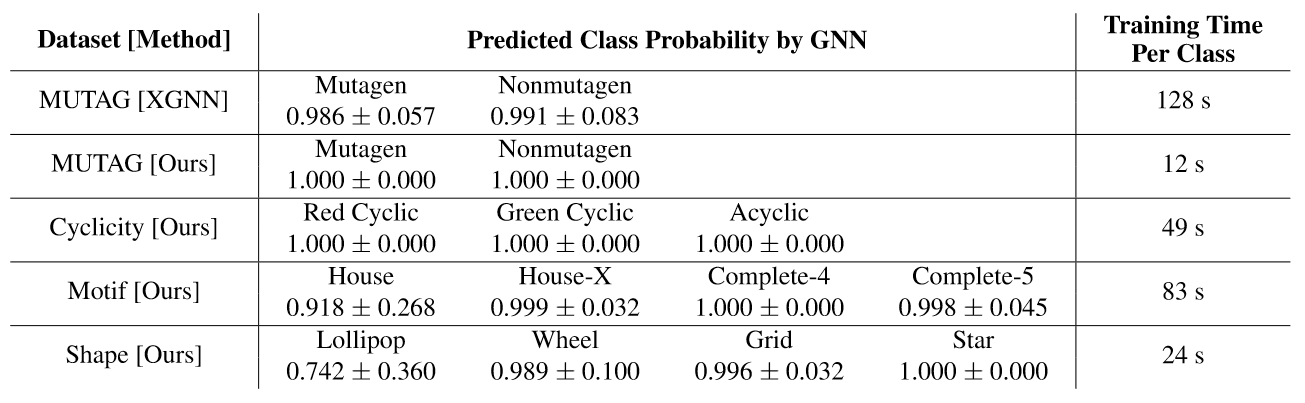
\includegraphics[width=0.9\textwidth,height=\textheight]{figures/GNNInt_prediction_results.png}

}

\caption{\label{fig-GNNInt-pred-results}A copy of the quantitative
modeling results from Table 2 in X. Wang and Shen
(\protect\hyperlink{ref-Wang_Shen_2024}{2024}).}

\end{figure}

\begin{figure}

{\centering 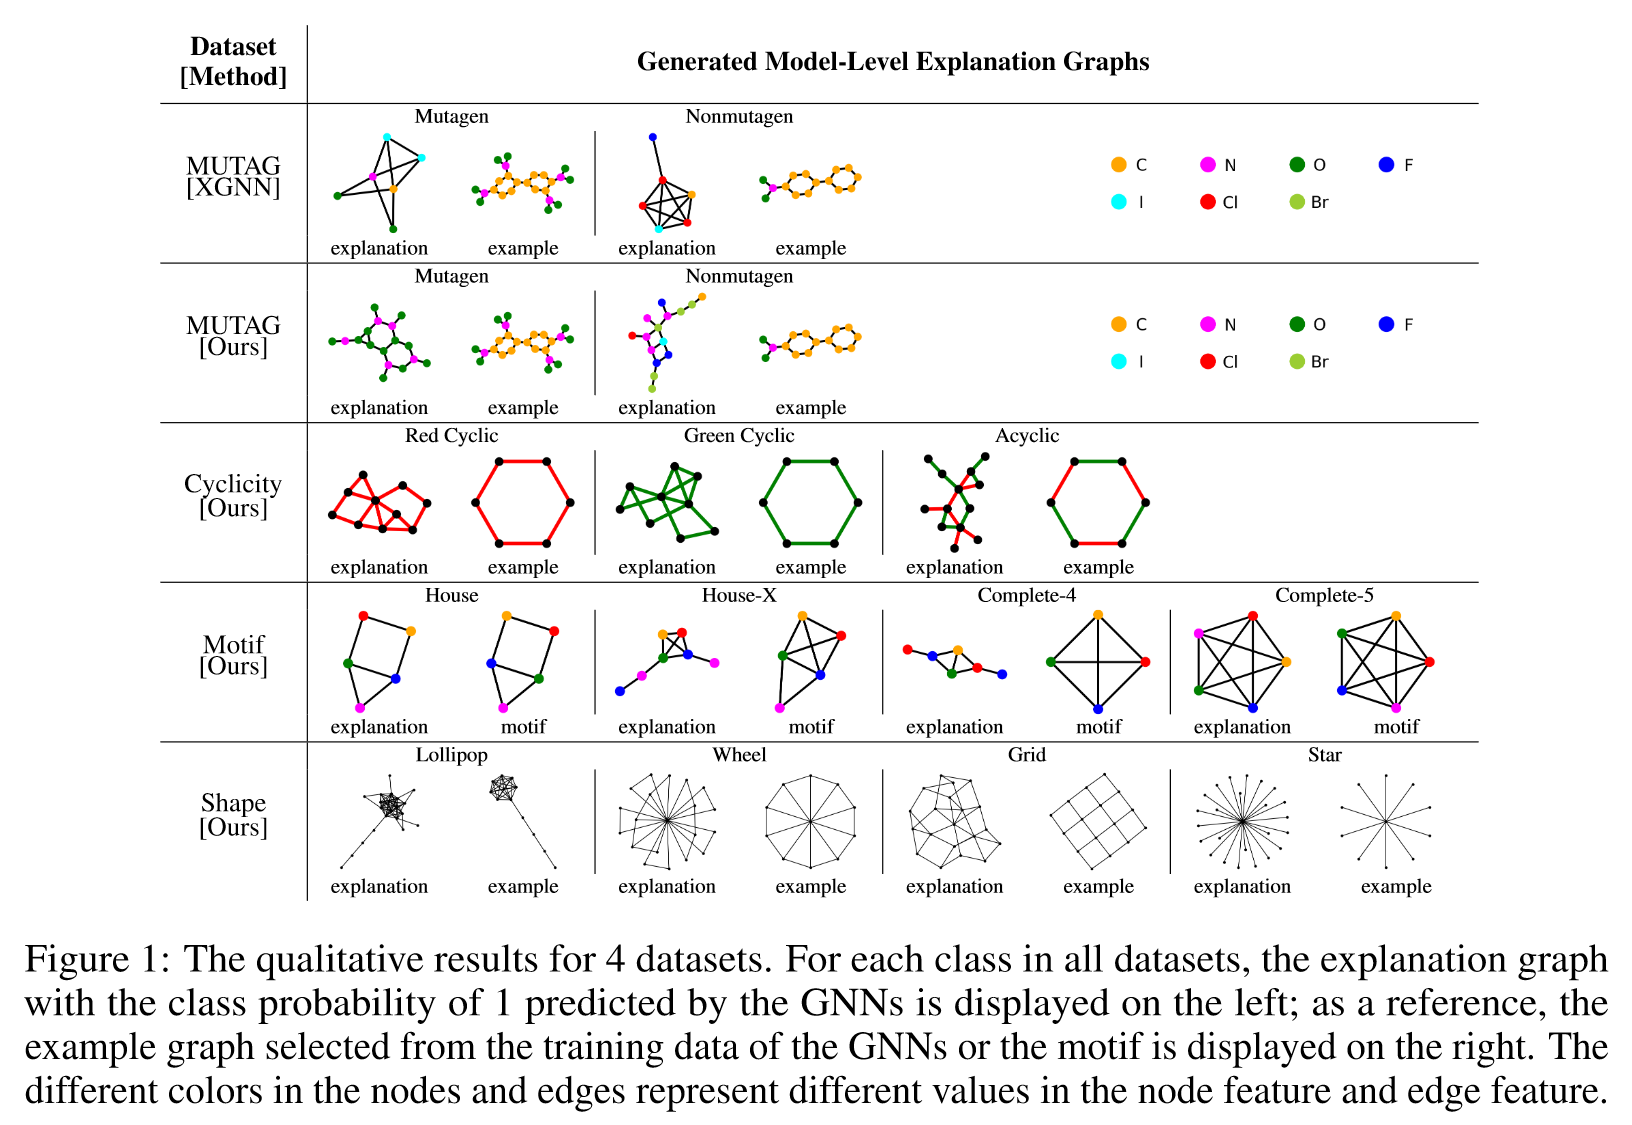
\includegraphics[width=0.8\textwidth,height=\textheight]{figures/GNNInt_drawn_results.png}

}

\caption{\label{fig-GNNInt-Drawn}A copy of the qualitative modeling
results from Figure 1 in X. Wang and Shen
(\protect\hyperlink{ref-Wang_Shen_2024}{2024}).}

\end{figure}

Qualitatively, Figure~\ref{fig-GNNInt-Drawn} displays limitations in
terms of realism. For instance, for the mutagen class, the explanation
correctly identifies the importance of the N02 group; however, the
generated graph is unrealistic and might not even be chemically
feasible. Additionally, the non-mutagen example lacks clear patterns or
identifiable structures. The explanations for the Cyclicity dataset, as
well as the Wheel and Grid classes, do not seem to be from their
respective underlying data distributions. In summary, GNNInterpreter
offers a method for generating example graphs that would be classified
as a targeted class by a GNN model, without requiring domain-specific
rules. However, optimizing for predictions and even embeddings alone
does not seem to be a sufficient objective for producing in-distribution
graphs. While the authors correctly note that focusing on predictions
can lead to unrealistic graphs, they also inadvertently show that
optimizing embeddings alone is not necessarily sufficient either.

\hypertarget{d4explainer-chen_wu_gupta_ying_2023}{%
\subsection{\texorpdfstring{D4Explainer
(\protect\hyperlink{ref-Chen_Wu_Gupta_Ying_2023}{Chen et al.
2023})}{D4Explainer (Chen et al. 2023)}}\label{d4explainer-chen_wu_gupta_ying_2023}}

\quad D4Explainer (\protect\hyperlink{ref-Chen_Wu_Gupta_Ying_2023}{Chen
et al. 2023}), or in-\textbf{D}istribution GNN Explanations via
\textbf{D}iscrete \textbf{D}enoising \textbf{D}iffusion, directly
addresses the realism of generated graphs in model-level explanations by
using a diffusion based generator model. In the image domain, diffusion
models have proven to produce more realistic images than other
generative AI methods, such as Generative Adversarial Networks (GANs).
These models work by iteratively adding noise to an observation until it
becomes pure noise. A denoising model is then trained to predict the
noise added at any step. New observations can be generated by reversing
this process, passing pure noise through the denoising model, a
technique known as reverse sampling. Additional objectives, such as a
desired class label, can be added to the loss function to generate
samples with certain properties.

\quad The authors here are focused on \emph{discrete structural
diffusion}. D4Explainer generate example graph by noising and denoising
the adjacency matrices of observed graphs. The sampled graphs have the
same features, but different structures. The process of gradually adding
noise to the input data is called \emph{forward diffusion}. Let
\(t \in [0, T]\) denote the current iteration. Let \(\beta_t\) be the
common probability that any edge changes state at time step \(t\).
\((\beta_1, \dots, \beta_T)\) is known as the variance schedule and is a
set hyperparameter. Let \(A_t\) be a one-hot encoded version of the
\(t^{th}\) noised adjacency. Then the forward diffusion process can be
expressed as:\\
\begin{equation}
         A_t[i, j] \sim q(A_t[i, \ j] \ | \ A_{t-1}[i, \ j]) 
            = \text{Cat}(A_{t-1}[i, \ j] \cdot Q_t)
    \end{equation} or \begin{equation} \label{eq-forward-diff}
         A_t[i, j] \sim q(A_t[i, \ j] \ | \ A_{0}[i, \ j]) 
            = \text{Cat}\left(A_0[i, \ j] \prod_{i=1}^t  Q_i \right)
    \end{equation} where, \[
    Q_t = 
    \left[
    \begin{matrix}
        1-\beta_t & \beta_t \\ 
        \beta_t & 1 - \beta_t
    \end{matrix}
    \right]
    \] the \(t^{th}\) element-wise transition matrix. The data need to
approach pure noise during the final iteration. This ensures that the
denoising model can start with pure noise. In the context of this
problem, a completely uninformative adjacency would be a Gilbert random
graph where the probability of any edge is 0.5. A proof of this property
for the above diffusion process is provide in Section~\ref{sec-proof}.

\quad Even though only the adjacency matrix is being noised, the authors
still wanted to use all of the available information during the
\emph{backwards diffusion} process. Thus the denoising model was
parameterized as: \begin{equation}
         p(A_0 \ | \ A_t, t, X_0, E_0; \ \Omega)  
    \end{equation} where \(\Omega\) is the set of trainable parameters.
The authors employed a \emph{Provably Powerful Graph Network} (PPGN)
(\protect\hyperlink{ref-Maron_Ben-Hamu_Serviansky_Lipman_2020}{Maron et
al. 2020}) as their denoising architecture; however, they have added an
additional neural network to learn the time or noise level effect. Like
most diffusion models, the primary objective is to minimize the distance
between the predicted denoised observation and the original. The authors
have added an additional weight term to focus the model on noisier or
more difficult training examples. The core loss function is expressed
as: \begin{equation} \label{L-dist}
        \mathcal{L}_{dist} (\Omega \ | \ A_0) =  \sum_{t=1}^T 
            \left(1 - 2 \bar \beta_t + \dfrac 1 T \right)
            \mathams{E}_{\hat A_0}
            \text{CrsEnt} \left(
                A_0, \hat A_0
            \right), 
    \end{equation} where
\(\hat A_0 = p(A_0 \ | \ A_t, t, X_0, E_0; \ \hat \Omega)\),
\(A_t[i, j] \sim q(A_t[i, \ j] \ | \ A_{0}[i, \ j])\), and \[
    \bar \beta_t = \frac 1 2 - \frac 1 2 \prod^t_{i=1}(1-2\beta_i), 
\]

the cumulative transition probability. After the denoising model has
been trained, model-level explanations are produced by iterative
sampling candidate adjacency structures for an observed set of graph
features and selecting the candidate with the highest probability of
being from the targeted class. This is a multi-step procedures, where at
each step \(A_t\) is denoised to \(k\) candidates \(A_0, 1 \dots k\).
The candidate with the best predicted probability is then noised to a
level of \(t-1\) and the process is repeated. The pseudocode is
reproduced below.

\begin{algorithm}
    \caption{D4Explainer Model-level Explanation Reverse Sampling Algorithm}\label{alg:cap}
    \begin{algorithmic}
        \Require $\hat \Omega$: trained denoising parameters; 
                $q(A_t \ | \ A_0)$: forward diffusion process.
        \renewcommand{\algorithmicrequire}{\textbf{Input:}}
        \renewcommand{\algorithmicensure}{\textbf{Output:}}
        \Require N: maximum number of nodes; T: maximum noise level; 
                K: number of candidates per iteration; 
                $\tilde{\rho}$ targeted prediction vector; 
                $(X, E)$: node and edge features.  
        \Ensure $\hat A$: adjacency matrix for model-level explanation.
        \State Sample $A_T[1:n, 1:n]$ \sim Bernoulli(0.5)
        \For{t in T to 1}
            \State Sample candidates 
                $\{\hat A_{0, k} \sim p(A_t,t, X, E; \ \hat \Omega) : k \in 1, \dots, K\}$
            \State Select the best candidate 
            $\underset{j \ \in \ i, \dots K}{\text{argmin}}$ 
            CrsEnt(explainee($G = (X, A_{0, j}, E)), \ \tilde{\rho}$)
            \State Sample $A_{t-1}[1:n, 1:n] \sim q(A_{t-1}, A_{0, j})$
        \EndFor
        \State \Return $A_0$
    \end{algorithmic}
    \end{algorithm}

\quad To assess how well a sampled explanation matches the observed
graph distribution, the authors compute various maximum mean discrepancy
(MMD) statistics. MMD is a general technique used to measure the
distance between two data distributions based solely on observed data.
The distributions are estimated using \emph{kernel density estimation},
and then the distance between their means is compared. As long as the
chosen kernel is \emph{characteristic}, an MMD statistics defined as the
l2 distance between \emph{kernel mean embeddings} is representative of
the distance between the true distributions
(\protect\hyperlink{ref-Gretton_Borgwardt_Rasch_Schuxf6lkopf_Smola_2012}{Gretton
et al. 2012}). The \emph{Gaussian Earth Mover's Distance kernel} was
selected here. The author use MMD statistics to compare the degree,
clustering, and spectrum distributions of the generated explanation
against the observed data. The degree distribution of a graph indicates
how frequently nodes have different numbers of connections, reflecting
the overall connectivity pattern. The clustering coefficient of a node
measures the proportion of the node's neighbors that are also connected
to each other, representing local clustering. The spectrum distribution,
which is the distribution of eigenvalues of the adjacency matrix or
Laplacian matrix, provides insights into the graph's structural
characteristics and dynamic properties. Similar to GNNInterpreter, the
author of D4Explainer also value the sparsity of their generate example.
They measure the density of a graph as the number of present edges
divided by the number of possible edges or \begin{equation}
        \text{Density} = \mathcal{|E|} / |\nu|^2. 
    \end{equation}

\quad In additional to model-level explanations, D4Explainer can provide
\emph{counterfactual explanations} by adding a term to the loss
function. The authors define a counterfactual explanation for a
particular observed graph to be \(G^c\) such that
\(\hat Y_{G^c} \neq \hat Y_G\), but the difference between \(G^c\) and
\(G\) is minimal. \(\mathcal{L}_{dist}\) (\ref{L-dist}) ensures that the
\(G^c\) generated does not stray too far from the observed graph
distribution, and adding \(\mathcal{L}_{CF}\) minimize the probability
that the generated graph is classified the same as the input.
\begin{equation}
         \mathcal{L}_{CF}(\Omega \ | \ A_0) = 
            \mathams{E}_{\hat A_0} - \log(1 - \rho_{G^c}[\hat Y_{G}]), 
    \end{equation} where \(G = (X, A, E)\) is an observed graph,
\(G^c = (X, \hat A_0, E)\), and \(\rho_{G^c}[\hat Y_{G}]\) denote the
probability that \(G^c\) belongs to the same class as \(G\). To quantify
the quality of generated counterfactual explanations, the author report
\emph{Counterfactual Accuracy}, \emph{Fidelity}, and \emph{modification
ratio}. CF-ACC measure the proportion of \(G^c\)s that have different
predicted labels than there associated observed graph.\\
\begin{equation}
            \text{CF-ACC} = \mathams{E}_{\hat A_0} \ I(\hat Y_{G^c} \neq \hat Y_{G}) 
    \end{equation}

Fidelity measures the difference in the predicted probability of \(G\)
and \(G^c\) with respected to the original class label.\\
\begin{equation}
        \text{Fidelity} = \mathams{E}_{\hat A_0} \ \rho_{G}[\hat Y_G] - \rho_{G^c}[\hat Y_G]
    \end{equation}

Finally, modification ratio measures difference in edges between \(G^c\)
and \(G\) relative to the size of the original graph.\\
\begin{equation} \label{mod-ratio}
        \text{MR} = \mathams{E}_{\hat A_0} \ \dfrac{|\sum_{i, j} A[i, j] - \hat A_0(i, j)|}{\sum_{i, j} A[i, j]}
    \end{equation}

\quad Similar to GNNInterpreter, the author report the mean predicted
probability for the targeted class. Using a maximum of 6 nodes, the
author were able to achieve a mean of 0.832 on the MUTAG dataset. Since
the counterfactual explanation are generated on a per observation basis,
the author's compared their method to other popular instance-level
explanation methods.

\begin{figure}

{\centering 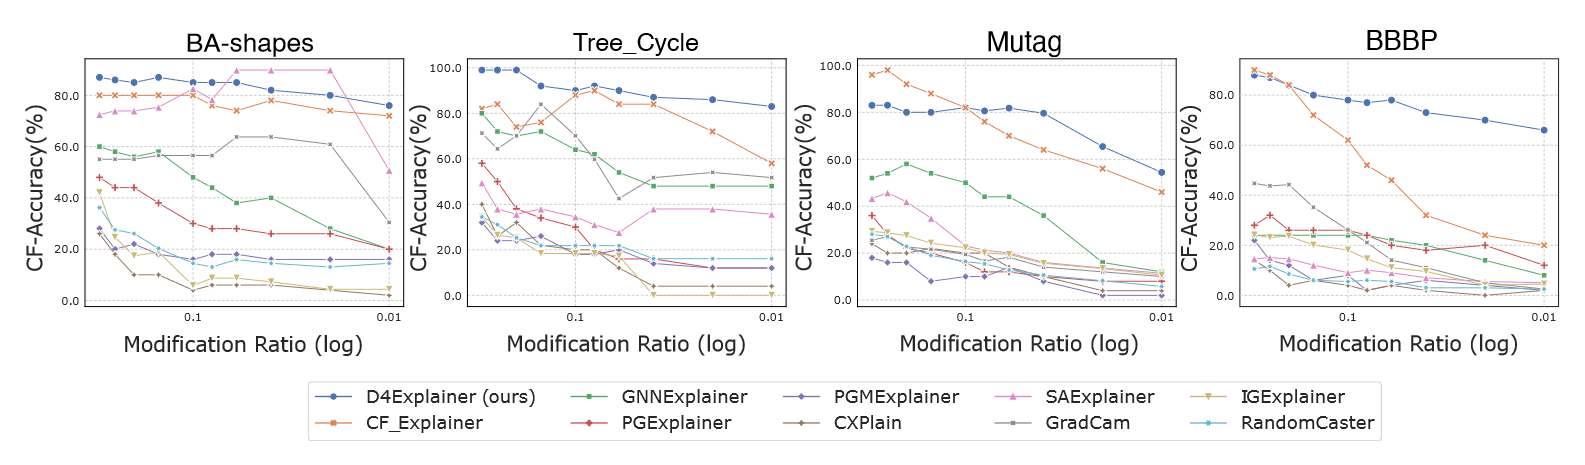
\includegraphics[width=0.9\textwidth,height=\textheight]{figures/D4-CF-Plot.png}

}

\caption{\label{fig-D4-CF-ACC}Comparison of the CF-ACC relative to MR of
various methods and datasets. A copy of Figure 4 from Chen et al.
(\protect\hyperlink{ref-Chen_Wu_Gupta_Ying_2023}{2023}).}

\end{figure}

Figure~\ref{fig-D4-CF-ACC} displays that D4Explainer can flip the
prediction on roughly 80\% of observed graphs at most modification
levels. Missing from the plot is a variance measure. It is possible that
the counterfactual accuracy varies more between different data splits or
hyperparameter than the other methods. Figure~\ref{fig-D4-MMD} indicates
that the D4Explainer generated graphs tend to have feature distributions
that are closer to the original dataset; however, there might be a
hidden class bias. The distributions might only be close for the
majority class, skewing the averages.

\begin{figure}

{\centering 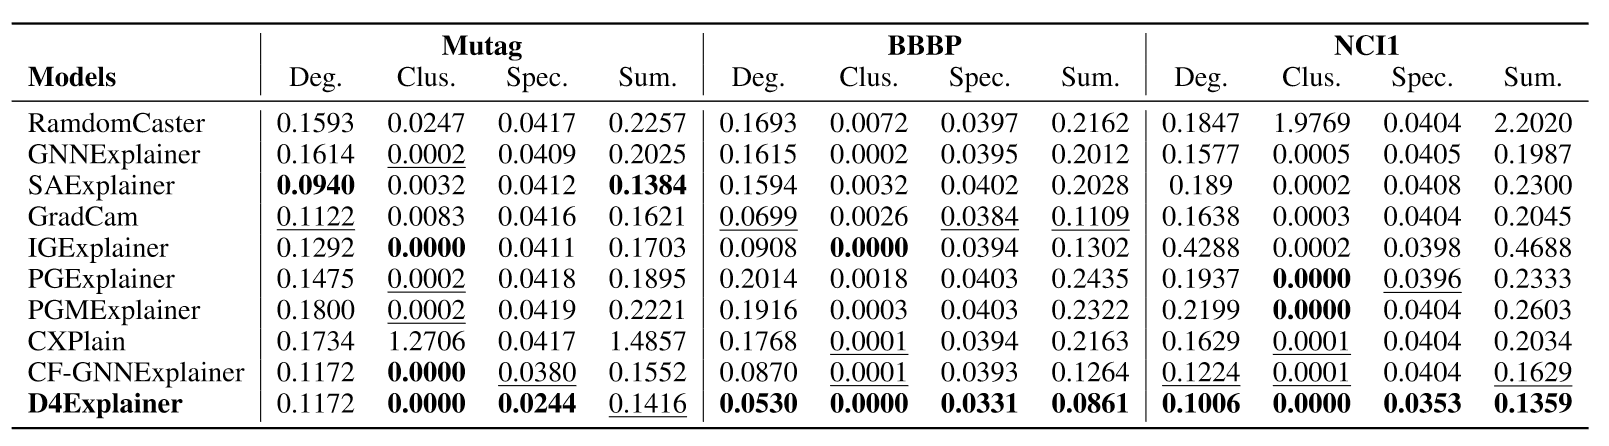
\includegraphics[width=0.9\textwidth,height=\textheight]{figures/D4-MMD-Table.png}

}

\caption{\label{fig-D4-MMD}MMD statistic for various methods and
datasets copied from Table 2 in Chen et al.
(\protect\hyperlink{ref-Chen_Wu_Gupta_Ying_2023}{2023}).}

\end{figure}

\hypertarget{protgnn-zhang_liu_wang_lu_lee_2021}{%
\subsection{\texorpdfstring{ProtGNN
(\protect\hyperlink{ref-Zhang_Liu_Wang_Lu_Lee_2021}{Zhang et al.
2021})}{ProtGNN (Zhang et al. 2021)}}\label{protgnn-zhang_liu_wang_lu_lee_2021}}

\quad Up until now, we have been discussing post-hoc explanation
methods; however, Rudin (\protect\hyperlink{ref-Rudin_2019}{2019})
raises two important concerns with this approach. First, parity in the
predictions does not guarantee parity in the reasoning. Explanations may
bear strong predictions, but for distinct and sometimes nonsensical
reasons. Recall that Figure~\ref{fig-random-baseline} showed that
completely random graphs can illicit confident predictions. Second,
feature importance indicates that a feature is significant to the model,
but it does not reveal how the model uses the feature. For instance, a
substructure might lead to a prediction due to a strong relation with
the target class, or it could be important because of a strong negative
relation with other classes. ProtGNN
(\protect\hyperlink{ref-Zhang_Liu_Wang_Lu_Lee_2021}{Zhang et al. 2021})
uses the prototype modeling paradigm to create a GNN that is
\emph{interpretable}. Prototype based models make prediction by
comparing new inputs to exemplar cases or \emph{learned prototypes} of
each class. This results in an interpretable model because, as long as
the prediction function applied to the prototype similarity scores is
simple, the reasoning for any given prediction will be clear.
Intuitively, this can be thought of as using a black-box model to
engineer features, which are then passed to a straightforward white-box
model.

\quad ProtGNN initializes \(m\) random prototype vectors for each of the
\(C\) classes. Let \(p_k\) denote a prototype vector and \(P_{Y_G}\)
denote the set of prototypes vectors assigned to the ground truth label
of \(G\), \(Y_G\). Now, let \(f(G; \ \Omega_f) = \hat p_G\) be a graph
encoder function that maps any graph into the prototype vector space,
where \(\Omega_f\) is the set of trainable parameters. \(f\) is
generally one of the standard GNN architectures. Since ProtGNN was
primarily designed to be a graph classification model, the author
optimized for predictive power using:\\
\begin{equation}
        \mathcal{L}_{\text{prot}}(\Omega_f, \ \Omega_\psi, \ p_1, \dots, p_{mC} \ | \ G)= \mathams{E}_G \ \text{CrsEnt} \left[\psi \left(sim\left(\hat p_G, p_1\right), \dots, sim\left(\hat p_G, p_{mC}\right); \ \Omega_\psi\right), \ Y_G \right]
    \end{equation} where \(\psi\) is any simple prediction model with
trainable parameters \(\Omega_\psi\) and \(sim\) is any vector
similarity function. ProtGNN uses a full connected layer with a softmax
output activation for \(\psi\), which is similar to a multinomial
regression model. To address similar out-of-distribution concerns
discussed earlier, the authors include three additional loss terms as
constraints. The cluster loss ensure that each embedding is close to at
least one prototype assigned to its ground truth class:\\
\begin{equation}
        \mathcal{L}_{\text{clst}}(\Omega_f, \ \Omega_\psi, \ p_1, \dots, p_{mC} \ | \ G) = \mathams{E}_G \ \underset{p_k \in P_{Y_G}}{\text{min}} || \hat p_G - p_k ||^2_2. 
    \end{equation} A separation loss ensures that embeddings are far
from the prototypes of other classes: \begin{equation}
        \mathcal{L}_{\text{sep}}(\Omega_f, \ \Omega_\psi, \ p_1, \dots, p_{mC} \ | \ G) = - \mathams{E}_G \ \underset{p_k \notin P_{Y_G}}{\text{min}} || \hat p_G - p_k ||^2_2. 
    \end{equation} Finally, the diversity loss encourages each prototype
within a class to learn different information:\\
\begin{equation}
            \mathcal{L}_{\text{div}}(\Omega_f, \ \Omega_\psi, \ p_1, \dots, p_{mC} \ | \ G) = \sum_{k=1}^C \sum_{p_i \neq p_j \in P_k} \ \max(0, cos(p_i, p_j) - s_\text{max})
    \end{equation} where \(s_\text{max}\) is a set similarity threshold.

\quad The learned prototypes are latent embedding vectors that are not
directly interpretable. To address this issue, the authors use a Monte
Carlo Tree Search (MCTS) algorithm
(\protect\hyperlink{ref-Coulom2006EfficientSA}{Coulom 2006}) to identify
the subgraph within the observed graphs of the prototype's class that
has an embedding closest to the given prototype. Specifically, the
author use the MCTS to select an optimal sequence of pruning actions.
Let \(\mathcal{G}_{0, \ i, \dots, j}\) represent the subgraph resulting
from the sequence of pruning actions
\(\text{act}_i,\dots, \text{act}_j\), where \(\mathcal{G}_0\), the root
of the search tree, is an observed graph. The MCTS algorithm proceeds in
4 core steps. First, an existing node in the search tree
\(\mathcal{G}_{0, \ i, \dots, j}\) is \emph{selected}. Second, the
chosen node is \emph{expanded} by adding a child node
\(\mathcal{G}_{0, \ i, \dots, j, k}\) resulting from action
\(\text{act}_k\). To limit the search space, the authors restrict
\(\text{act}_k\) to be the removal of a peripheral node with minimum
degree. Third, the reward for the sequence of actions \(i, \dots, j, k\)
is estimated via a Monte Carlo \emph{simulation} where additional random
actions are taken until a subgraph of the desired size is produced. The
sampled embeddings are then compared to the prototype vector and the
similarities are averaged. Finally, the child node's estimated score is
then \emph{backpropagated} to update the estimated scores of all its
parent nodes. After a fixed number of iterations through the observed
graphs from the prototype's class, the decision path with the highest
resulting score is selected to produce the ultimate prototype
projection. In addition to finding the closest subgraph in the observed
class, the authors also suggest a method for finding similar subgraphs
within each input. This is done by training a neural network to predict
an edge mask conditional on a prototype vector:\\
\begin{equation}
        \hat A[i, \ j] = \text{nn}\left(G, p_k; \ \Omega_{\text{nn}}\right).  
    \end{equation}

The resulting induced subgraph's embedding, \(\hat p_{G_k}\), are then
optimized to be as close as possible to the given prototype:
\begin{equation}
        \mathcal{L}(\Omega_{\text{nn}}, \ \Omega_f, \ p_k \ | \ G) = -\mathams{E}_G \ sim(\hat p_{G_k}, p_k). 
    \end{equation}

The authors denote the version of the model that utilizes this
\emph{conditional subgraph sampling module} as \textbf{ProtGNN+}.

\quad ProtGNN achieves similar or better graph classification accuracy
than state of the art models across 5 standard benchmark datasets (see
Figure~\ref{fig-prot-acc-table}).

\begin{figure}

{\centering 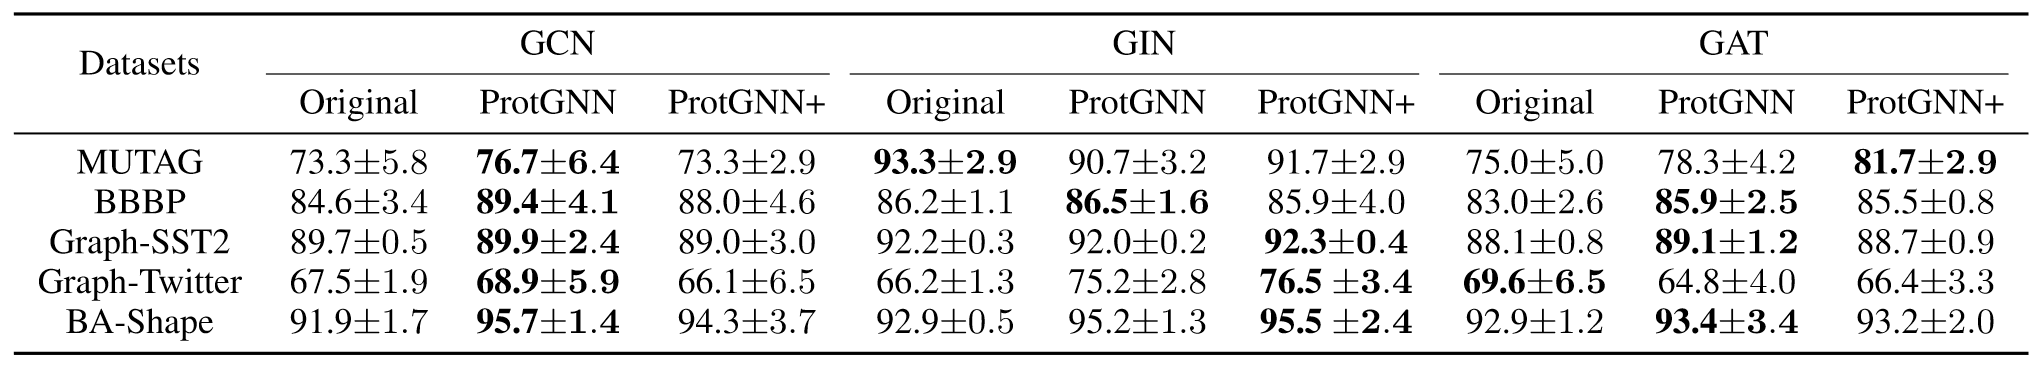
\includegraphics[width=0.9\textwidth,height=\textheight]{figures/prot_acc_table.png}

}

\caption{\label{fig-prot-acc-table}A copy of the quantitative modeling
results report in Table 1 of Zhang et al.
(\protect\hyperlink{ref-Zhang_Liu_Wang_Lu_Lee_2021}{2021}).}

\end{figure}

Figure~\ref{fig-prot-acc-table} also indicates that ProtGNN is robust to
the choice of embedding model as there seems to be benefits across
various GNN architectures. The authors do note that the computational
complexity of ProtGNN can be significantly higher than a standard GNN
model, taking roughly 5 times longer to train. Most of this complexity
is attributable to the use of the MCTS. On the other hand, ProtGNN
allows for easier and clearer inference. Figure~\ref{fig-prot-diagram}
demonstrates that the output of ProtGNN is similar to a simple
regression model. The prototypes can be thought of as features, the
similar subgraphs and similarity scores as the observed feature values,
and the class connections as the marginal effects on the prediction.

\begin{figure}

{\centering 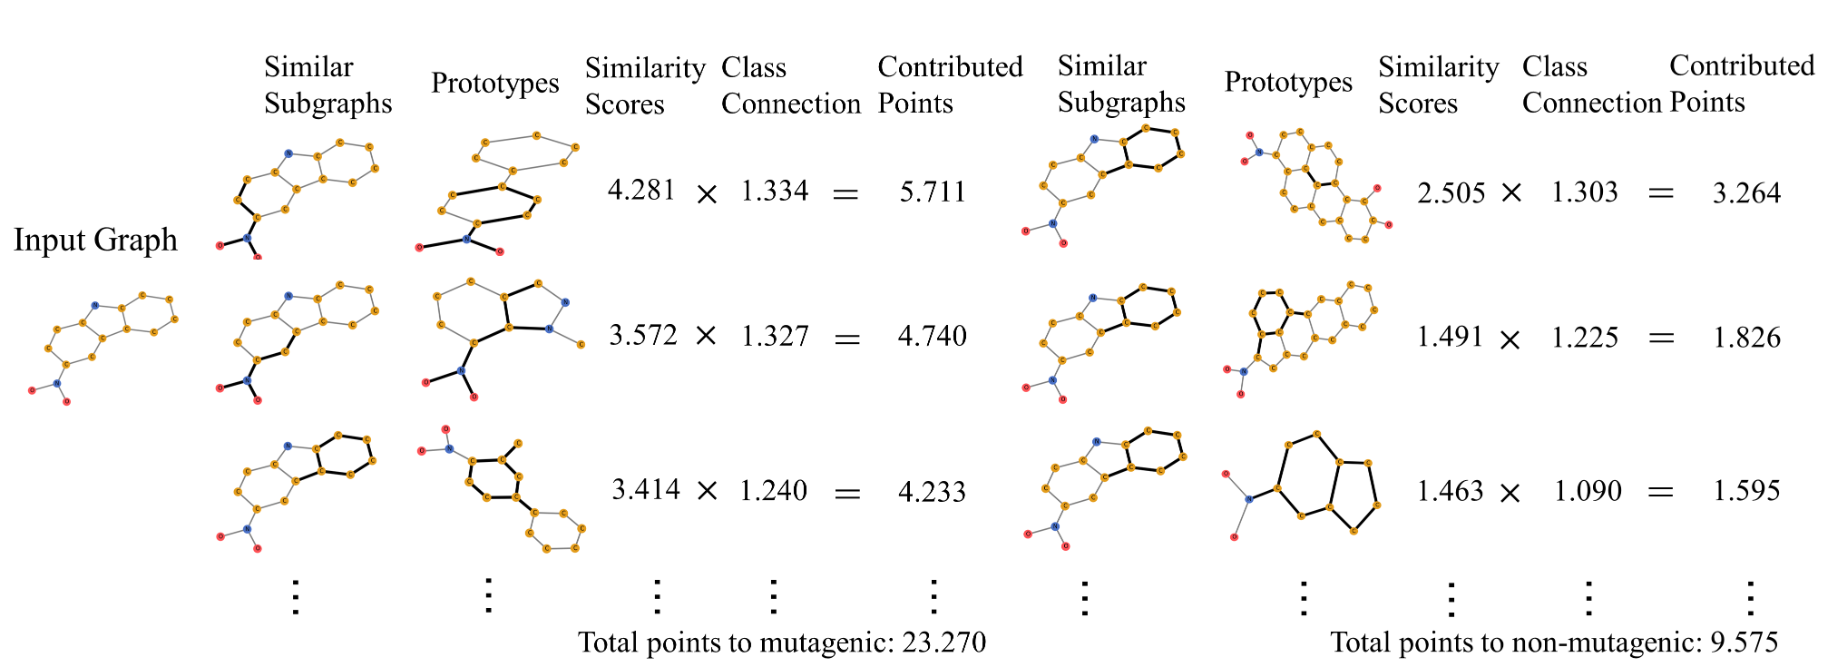
\includegraphics[width=0.9\textwidth,height=\textheight]{figures/prot_inference_ex.png}

}

\caption{\label{fig-prot-diagram}An example ProtGNN+ output for the
MUTAG dataset taken from Figure 3 in Zhang et al.
(\protect\hyperlink{ref-Zhang_Liu_Wang_Lu_Lee_2021}{2021}).}

\end{figure}

Since prototypes from every class are used for the classification,
ProtGNN can also be used for counterfactual type analysis. For any given
predictions, researcher can determine why a certain classification was
made and why the other classes were not selected.
Figure~\ref{fig-prot-diagram} display both a strong similarity to the
mutagenic prototypes as well as a weaker relation to the non-mutagenic
prototypes.

\hypertarget{synthesis-of-core-papers}{%
\section{Synthesis of Core Papers}\label{synthesis-of-core-papers}}

\quad GNNInterpreter and D4Explainer are both \emph{post-hoc generative
explanation methods}. Each defines a model-level explanation for a given
class \(c\) as an estimated graph generating distribution:\\
\begin{equation}
        G_\text{Gen, c} \sim f(G \ | \ \Theta) \text{ subject to } \underset{\Theta}{\text{argmin}}\ \mathams{E}_{G_\text{Gen}} \ \text{CrsEnt}\left[\text{explainee}(G_\text{Gen}), \ \tilde{\rho_c}\right].
    \end{equation}

In other words, an explanation is the distribution that maximizes the
probability that a sampled graph will be classified by the
\emph{explainee} as the desired class \(c\). The key difference between
the methods is the form of \(f(G \ | \ \Theta)\). This is akin to the
parametric or distributional assumption for classical statistical
methods. GNNInterpreter assumes that each graph matrix has a separate
distribution with possibly dependent parameters. On the other hand,
D4Explainer assumes that the only random variation between graphs is in
the adjacency structure. Both models assume that every entry of the
adjacency matrix follows a Bernoulli distribution, but diverge in terms
of estimating the probability. The methods also utilize different
sampling procedures. GNNInterpreter clearly estimates the distributional
parameters and samples traditionally. In contrast, D4Explainer employs a
black-box denoising model. D4Explainer makes use of the observed graphs
directly, whereas GNNInterpreter only injects latent embeddings. This
makes GNNInterpreter much more sensitive to the underlying explainee
model.

\quad Both sets of authors highlight the \emph{out-of-distribution}
problem that plagues generative explanations. GNN models are not robust
to out-of-distribution or unrealistic graphs, which is to say that
explainee models can still return a confident classification for a
complete random graph (see Figure~\ref{fig-random-baseline}).
D4Explainer partial resolves this issue by restricting generated node
and edge features to the observed values. This ensures that the features
of any generated graph will not be out-of-distribution; however, this
limits inference. GNNInterpreter tackles the problem by optimizing the
similarity to the average class embedding; however, embeddings can also
suffer from out-of-distribution problems
(\protect\hyperlink{ref-Steck_Ekanadham_Kallus_2024}{Steck, Ekanadham,
and Kallus 2024}). Just as an unrealistic or random graph can yield
similar predictions, it can also have similar embeddings due to
information loss in the lower-dimensional space (see Table
\ref{tab-sim}). While GNNInterpreter and D4Explainer place differing
restrictions on their respective likelihoods, the terms are
interchangeable. For example, there is no reason why
\(\mathcal{L}_\text{spars}\) (\ref{l-spars}) could not be included in
the loss for D4Explainer. Similarly, the MMD statistics from D4Explainer
could be used to evaluate graphs generated from GNNInterpreter (see
Table \ref{tab-results}).

\quad ProtGNN, unlike the first two methods, is a \emph{self
interpretable GNN model}. Rather than attempting to decipher a
predictive model, ProtGNN itself serves as the predictive model.
Prototype similarity is closely related to GNNInterpreter's
\(\mathcal{L}_\text{embed}\) (\ref{l-embed}) as they both measure the
similarity between graphs in a latent vector space; however, unlike
GNNInterpreter, the embedding function in ProtGNN is trainable.
Furthermore, ProtGNN also uses dissimilarity to the non-target classes,
but this could be easily added to GNNInterpreter's loss. On the other
hand, similar to D4Explainer, the graph projections created from the
prototype are restricted to the observed data. It is also worth
distinguishing that the similar subgraphs created by ProtGNN+ are
instance-level explanations, while the class connection weights and
prototype projections are model-level. D4Explainer produces
counterfactual examples be directly computing possible input changes
that could flip the prediction, while ProtGNN demonstrates how the
prediction could have changed by display the similarity to structures
indicative of other classes. While not the traditional directly
counterfactual analysis, ProtGNN provides model-level insight.

\quad Experts in the field seem to agree that a class-conditional
graph-generating distribution would help illuminate the black-box nature
of GNNs. However, there is no consensus on the ideal form or likelihood
of such a distribution. While diffusion has proven to be a strong
generative method in other applications, D4Explainer's feature
restriction and convoluted sampling algorithm leave much to be desired.
The results from GNNInterpreter suggest that conditional denoising might
be superior. Specifically, optimizing for prediction accuracy tends to
produce better intervals, with GNNInterpreter achieving 1.0 (see
Figure~\ref{fig-GNNInt-pred-results}) compared to D4Explainer's 0.832 on
the MUTAG dataset. Explicit prototype-based models are fairly uncommon
in the literature, but we believe most researchers would agree that
Figure~\ref{fig-prot-diagram} provides very clear inference. On the
other hand, completely refactoring the predictive model is not always
feasible, so both explainable and interpretable GNN methods remain
important research avenues.

\hypertarget{technical-details}{%
\section{Technical Details}\label{technical-details}}

\hypertarget{methodology}{%
\subsection{Methodology}\label{methodology}}

\quad Since GNNInterpreter only makes qualitative assessments of
generated structures, we applied the metrics describe in D4Explainer to
quantify the properties of the generating distribution. We reimplemented
GNNInterpreter using an identical generation scheme and loss function.
We trained the reimplemented model on the MUTAG
(\protect\hyperlink{ref-Debnath_1991}{Debnath et al. 1991}), a standard
benchmark graph classification dataset. MUTAG consists of nitroaromatic
compounds, with the goal being to predict their mutagenicity on
Salmonella typhimurium. Each observation is a graphs representing a
chemical structure, where vertices denote atoms and edges represent
bonds. For our explainee model, we also implemented a 3-layer GCN model.
There are slight variations between the architectures and training
hyperparameters, but the accuracies are comparable, 86\% (ours) and 92\%
(theirs). We additionally reimplement D4Explainer's counterfactual
generator. Although not discussed in the original paper, this model can
also be used to produce model level explanations. We simply randomly
sample a graph from the opposite class and take the generated counter
factual graph as our explanation.

\hypertarget{results}{%
\subsection{Results}\label{results}}

\begin{longtable}[t]{llllll}
\caption{Comparison of Original and Reimplement Model Results.} \label{tab-results} \\
\toprule
  & Predictions & Density & Deg. & Clus. & Spec.\\
\midrule
\addlinespace[0.3em]
\multicolumn{6}{l}{\textbf{GNNInterpreter Original}\textsuperscript{2}}\\
\hspace{1em}Class 0 & 1.0 +/- 0.0 & NA & NA & NA & NA\\
\hspace{1em}Class 1 & 1.0 +/- 0.0 & NA & NA & NA & NA\\
\addlinespace[0.3em]
\multicolumn{6}{l}{\textbf{GNNInterpreter Reimplemented}}\\
\hspace{1em}Class 0 & 0.93 +/- 0.01 & 0.38 +/- 0.002 & 1.77 & 1.53 & 0.07\\
\hspace{1em}Class 1 & 0.98 +/- 0.01 & 0.32 +/- 0.003 & 1.41 & 1.43 & 0.04\\
\addlinespace[0.3em]
\multicolumn{6}{l}{\textbf{D4Explainer Original}}\\
\hspace{1em}Aggregated & 0.92\textsuperscript{2} & 0.315\textsuperscript{2} & 0.12\textsuperscript{3} & 0.00\textsuperscript{3} & 0.02\textsuperscript{3}\\
\addlinespace[0.3em]
\multicolumn{6}{l}{\textbf{D4Explainer Reimplemented}}\\
\hspace{1em}Class 0 & 0.63 +/- 0.23 & 0.13 +/- 0.03 & 0.27 & 0.57 & 0.05\\
\hspace{1em}Class 1 & 0.66 +/- 0.20 & 0.13 +/- 0.03 & 0.08 & 0.25 & 0.04\\
\bottomrule
\multicolumn{6}{l}{\rule{0pt}{1em}\textsuperscript{1} +/- 1 standard deviation; 1,000 sample graphs.}\\
\multicolumn{6}{l}{\rule{0pt}{1em}\textsuperscript{2} From Table 2 in Wang and Shen (\protect\hyperlink{ref-Wang_Shen_2024}{2024}).}\\
\multicolumn{6}{l}{\rule{0pt}{1em}\textsuperscript{2} From Table 3 in Chen et al.
(\protect\hyperlink{ref-Chen_Wu_Gupta_Ying_2023}{2023}).}\\
\multicolumn{6}{l}{\rule{0pt}{1em}\textsuperscript{2} From Table 2 in Chen et al.
(\protect\hyperlink{ref-Chen_Wu_Gupta_Ying_2023}{2023}).}\\
\end{longtable}

\begin{figure}

{\centering 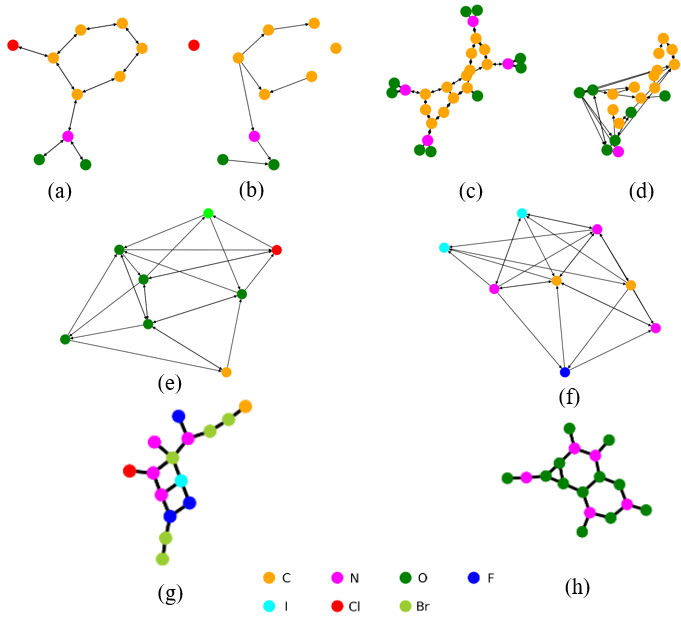
\includegraphics[width=1\textwidth,height=1\textheight]{figures/mutag_plot_together.png}

}

\caption{\label{fig-results}(a) Observed graph from class 0, Pr = 0.92;
(b) Generated counterfactual explanation of (a) from D4Explainer
reimplemented, Pr = 0.67; (c) Observed graph from class 1, Pr = 0.96;
(d) Generated counterfactual explanation of (b) from D4Explainer
reimplemented, Pr = 0.96; (e) Generated explanation for class 0 from
GNNInterpreter reimplemented, Pr = 0.94; (f) Generated explanation for
class 1 from GNNInterpreter reimplemented, Pr = 1.0; (g) Generated
explanation for class 0 from GNNInterpreter (X. Wang and Shen
(\protect\hyperlink{ref-Wang_Shen_2024}{2024}), Figure 1, pg.7), Pr =
1.0; (h) Generated explanation for class 1 from GNNInterpreter (X. Wang
and Shen (\protect\hyperlink{ref-Wang_Shen_2024}{2024}), Figure 1,
pg.7), Pr = 1.0.}

\end{figure}

\quad We were unable to replicate GNNInterpreter's 0 variance predictive
accuracy, but the values are comparable given the lack of extensive
hyperparameter tuning (see Table \ref{tab-results}). The predictions are
similarity superior to the original D4Explainer results, 0.93 and 0.98
v. 0.92. As noted by the authors, the explainee model has a bias towards
the mutagenic class (class 1), which can explain the greater deviation
between the class 0 models. Another limiting factor is a lower set
maximum number of nodes. We set it to 8 to make the results more
comparable to the model-level explanation reported by D4Explainer.
Surprisingly, D4Explainer produces sparser graphs than GNNInterpreter in
terms of average density, 0.38 and 0.32 v. 0.315. This is despite the
fact that D4Explainer has no explicit penalty in the loss function.
Based on the MMD statistics, D4Explainer produces graphs with better
in-distribution properties (see \ref{tab-results}). This might be due to
the explicit regularization in GNNInterpreter, as penalizing the edge
probabilities could lead to a different degree distribution.
Additionally, the clustering coefficient might be affected, since fewer
edges result in fewer triangle clusters. The spectrum distributions are
similar for both models, as both enforce similarity in the explainee
embedding space, which aligns with the nature of the spectrum
distribution. However, one could argue that having a similar degree
distribution and clustering coefficient may not always be desirable. For
larger or more densely connected graphs, lower MMD statistics might
result in explanations that are too complex to be useful.

\quad Similar to the original examples display in GNNInterpreter, the
generated non-mutagenic graphs do not have clear or realistic structures
(see Figure~\ref{fig-results}). Graph (f) highlights that nitrogen in
key. We believe that this result is consistent with the original
findings about the N02 groups, but because of the more restrictive node
limit, our reproduction focuses on nitrogen since multiple oxygens can
be found in non-mutagenic chemicals. The reimplemented D4Explainer has a
CF-ACC in line with the original paper, 76.32\% at 0.41 log MR (see
Figure~\ref{fig-D4-CF-ACC} for the original metrics). The reimplemented
D4Explainer produces the least dense graphs, but has the least
discriminative predictions. The latter makes sense, since the goal of
the counterfactual loss is to flip the prediction, not necessarily
maximize confidence. One the other hand, this model demonstrates that it
is possible to generate sparse graphs with similar degree and clustering
distributions. Visually the counterfactual explanation make sense. Graph
(b) eliminated the red or chlorine atom which is typically associated
with non-mutagenic compounds
(\protect\hyperlink{ref-Yuan_Tang_Hu_Ji_2020}{Yuan et al. 2020}). Graph
(d) corrupted 3 of the 4 N02 groups, which is in line with
GNNInterpreter's findings that multiple N02 groups is a strong indicator
of mutagenicity.

\quad These results point to two main conclusions. First, the generator
model should make use of graph level data. GNNInterpreter uses
information about the graph structure through the explainee, but never
on the raw scale. This lack of graph level information can result in
unrealistic distributional properties. One way of including this
information would be to use the observed graphs to help predict the
distributional parameters. Alternatively, the generator could be
replaced with a diffusion model without any modififcation to the loss.
Second, the generator model should use class or prediction information.
D4Explainer's model-level sampling algorithm is less efficient and less
accuracate than GNNInterpreter's direct optimization during training.
The modified sampling algorithm demonstrates that single-step denoising
can still maintain low MMD statistics. Adding
\(\mathcal{L}_\text{pred}\) (\ref{l-pred}) and/or
\(\mathcal{L}_\text{embed}\) (\ref{l-embed}) could further improve this
type of sampling. Alternatively, a class label embedding, similar to the
time embedding, could be included to establish a conditional diffusion
model, which has worked extremely well in other applications.
Additionally, it would be easy to explore diffusing the node and edge
features as these types of models already exist
(\protect\hyperlink{ref-Vignac_Krawczuk_Siraudin_Wang_Cevher_Frossard_2023}{Vignac
et al. 2023}).

\hypertarget{sec-proof}{%
\subsection{Proofs}\label{sec-proof}}

\textbf{Proof of Equation \ref{gumbel-max-eq}:} WLOG assume we want to
sample for a categorical distribution \(\text{cat}(\theta_\text{cat})\)
with a set of \(W\) categories each with a probability \[
\pi_\omega = \dfrac{\theta_\text{cat}[\omega]}{\sum_{i \in W}\theta_\text{cat}[i]}.
\]

Define random variable \[
D = \text{argmax} \ \log \theta_\text{cat} + \text{Gumbel}(0, 1) = \underset{i \in W}{\text{argmax}} \ \log \theta_\text{cat}[i] + \text{Gumbel}(0, 1)[i], 
\]

here \(\text{Gumbel}(0, 1)[i]\) denotes the \(i^{th}\) i.i.d. sample
from the associated Gumbel. In order for \(D\) to be a true categorical
random variable, \(Pr[D = \omega]\) need to be \(\pi_\omega\).
\(D = \omega\) if and only if
\(\log \theta_\text{cat}[\omega] + \text{Gumbel}(0,1)[\omega] > \log \theta_\text{cat}[i] + \text{Gumbel}(0, 1)[i] \ \forall i \in W \setminus \omega\).
Now, let \(M_i\) denote a random variable that follows a
\(\text{Gumbel}(\log \theta_\text{cat}[i], 1)\) distribution. Then,
\begin{align*}
        Pr[D = \omega] 
            &= \mathams{E}_{M_\omega} 
                \prod_{i \in W \setminus \omega} Pr(M_i < m_\omega) 
                \text{ i.i.d location shifted Gumbel distributions.} \\ 
            &= \mathams{E}_{M_\omega} 
                \prod_{i \in W \setminus \omega} \exp 
                    \left(-e^{\log \theta_\text{cat}[i] - m_\omega} \right)
                \text{ Gumbel CDF.} \\ 
            &= \mathams{E}_{M_\omega} 
                \exp \left(-\sum_{i \in W \setminus \omega}
                e^{\log \theta_\text{cat}[i] - m_\omega} \right) \\ 
            &= \int_{-\infty}^{\infty}
                \exp \left( \log \theta_\text{cat}[\omega] - m_\omega \right) 
                \exp \left(-e^{\log \theta_\text{cat}[\omega] - m_\omega} \right) \cdot 
                \exp \left (-\sum_{i \in W \setminus \omega}
                e^{\log \theta_\text{cat}[i] - m_\omega} \right) \ dm \\
                &\text{ Gumbel PDF.} \\
            &= \int_{-\infty}^{\infty}
                \exp \left( \log \theta_\text{cat}[\omega] - m_\omega \right) 
                \exp \left (-\sum_{i \in W}
                e^{\log \theta_\text{cat}[i] - m_\omega} \right) \ dm \\
            &= \int_{-\infty}^{\infty}
                \theta_\text{cat}[\omega] 
                \exp \left( -m_\omega \right) 
                \exp \left( -e^{-m_\omega} \sum_{i \in W}
                    \theta_\text{cat}[i]  \right) \ dm \\
            &= \pi_\omega \sum_{i \in W} \theta_\text{cat}[i]
            \int_{-\infty}^{\infty}
                \exp \left( -m_\omega \right) 
                \exp \left( -e^{-m_\omega} \sum_{i \in W}
                    \theta_\text{cat}[i]  \right) \ dm 
                    \text{ From the above definition of } \pi_\omega \\
            &= \pi_\omega \sum_{i \in W} \theta_\text{cat}[i]
                \dfrac{\exp\left( -e^{-m_\omega} \sum_{i \in W} \theta_\text{cat}[i] \right)
                    }{\sum_{i \in W} \theta_\text{cat}[i]} \bigg|_{-\infty}^\infty \\ 
            &= \pi_\omega \sum_{i \in W} \theta_\text{cat}[i]
                \dfrac{1}{\sum_{i \in W} \theta_\text{cat}[i]} = \pi_\omega. 
    \end{align*} Reference: Huijben et al.
(\protect\hyperlink{ref-Huijben_Kool_Paulus_van_Sloun_2022}{2022})

\textbf{Proof of the limiting property of \ref{eq-forward-diff}:}
\begin{align*}
         \lim_{t \to \infty} q(A_t[i, \ j] \ | \ A_{t-1}[i, \ j]) 
            &= \lim_{t \to \infty} \text{Cat}\left(A_0[i, \ j] \prod_{i=1}^t Q_i \right) \\
            &= \lim_{t \to \infty} \text{Cat}
            \left(A_0[i, \ j] 
                \prod_{i=1}^t  
                \left[
                \begin{matrix}
                    1  & -1 \\
                    1 & 1
                \end{matrix}
                \right]
                \left[
                \begin{matrix}
                    1  &  0 \\
                    0 & 1-2\beta_i
                \end{matrix}
                \right]
                \left[
                \begin{matrix}
                    0.5  &  0.5 \\
                    -0.5 & 0.5
                \end{matrix}
                \right]
            \right) \\ 
            &\text{Eigen decomposition.} \\ 
            &= \lim_{t \to \infty} \text{Cat}
            \left(A_0[i, \ j] 
                \left[
                \begin{matrix}
                    1  & -1 \\
                    1 & 1
                \end{matrix}
                \right]
                \left[
                \begin{matrix}
                    1  &  0 \\
                    0 & \prod_{i=1}^t 1-2\beta_i
                \end{matrix}
                \right]
                \left[
                \begin{matrix}
                    0.5  &  0.5 \\
                    -0.5 & 0.5
                \end{matrix}
                \right]
            \right) \\ 
            &= \text{Cat}
            \left(A_0[i, \ j] 
                \left[
                \begin{matrix}
                    1  & -1 \\
                    1 & 1
                \end{matrix}
                \right]
                \left[
                \begin{matrix}
                    1  &  0 \\
                    0 & 0
                \end{matrix}
                \right]
                \left[
                \begin{matrix}
                    0.5  &  0.5 \\
                    -0.5 & 0.5
                \end{matrix}
                \right]
            \right) \\ 
            &\text{Set }\beta < 0.5. \\
            &= \text{Cat}
            \left(A_0[i, \ j] 
                \left[
                \begin{matrix}
                    0.5 & 0.5 \\
                    0.5 & 0.5
                \end{matrix}
                \right]
            \right) \\ 
            &= \text{Cat}([0.5, 0.5]) = \text{Bernoulli}(0.5)
    \end{align*}

\hypertarget{future-directions}{%
\section{Future Directions}\label{future-directions}}

\hypertarget{graph-edit-distance}{%
\subsection{Graph Edit Distance}\label{graph-edit-distance}}

\quad GNNInterpreter generates graphs with predictions very close to the
target class, but lack good in-distributions properties. D4Explainer, on
the other hand, generates explanations with more consistent features
distributions, but the predicted probabilities display higher variance.
Furthermore, while the model parameters of GNNInterpreter's generator
can be interpreted, D4Explainer introduces another black-box model. We
propose using a \textbf{differentiable approximation to the graph edit
distance (GED)} as a way of generically enforcing structural
consistency. GED measures the similarity between two graphs by counting
the minimum number of edits required to make the graphs isomorphic or
subgraph isomorphic. GED is similar to the modification ratio for
counterfactual explanations (see Equation \ref{mod-ratio}). Edit
distance has the key advantage of being human interpretable. For
example, the percentage of atoms and bonds that need to be changed for
two molecules to match is more relatable than the cosine distance
between their embeddings. Finding the exact optimal GED is a known
NP-complete problem, and most solutions are not differentiable
(\protect\hyperlink{ref-Bougleux_Brun_Carletti_Foggia_Gauxfczuxe8re_Vento_2015}{Bougleux
et al. 2015}). Fortunately, approximating GED as a quadratic assignment
problem (QAP) solves both the time complexity and derivative issue
(\protect\hyperlink{ref-wang2024pygm}{R. Wang et al. 2024}).

\quad Let \(G_1\) and \(G_2\) be graphs we wish to compute the GED
between. QAP approximates this be solving the following optimization
problem: \begin{equation} \label{QAP-obj}
    \mathcal{L}_{\text{GED}}(G_1, G_2) = \underset{M}{\max} \ \text{vec}(M) \ K(G_1, G_2) \ \text{vec}(M)^T.
\end{equation}

Here \(M\) is a \((n_1 \times n_2)\) binary node matching matrix and
\(K\) is a \((n_1 n_2 \times n_1 n_2)\) quadratic affinity matrix that
encode both node and edge similarities. The efficiency of QAP comes from
the fact that when any two nodes are matched together, the above
objective will account for the possible edges that could connect the
nodes. In order for the solution to be interpreted as an edit distance,
each entry of \(K\) should range from {[}-1, 0{]}, where -1 signals the
need for a complete edit and 0 means no edits are required
(\protect\hyperlink{ref-wang2024pygm}{R. Wang et al. 2024}). We suggest
the following similarity metric for every pair of nodes and edges:
\begin{equation}
    \begin{split}
         &-\lambda_1 \left[ 1 - \phi(\text{Continuous Features}) \right] \ + \\
         &-\lambda_2 \left[1 - \phi(\text{Discrete Features}) \right], 
    \end{split}
\end{equation}

where \(\phi(.)\) is the normalized cosine distance. \(1 - \phi(.)\)
will return 2 is the vectors are in opposite directions, 1 if the
vectors are orthogonal, and 0 if they are pointing in the same
direction; however, one-hot encoded vectors will never be in opposite
directions, so the different types of feature must be weighted
accordingly. Computing affinity this way allows for \(K\) to be
differentiable w.r.t. generated graph features. Furthermore we suggest
using the reweighted random walks algorithm
(\protect\hyperlink{ref-Cho_Lee_Lee_2010}{Cho, Lee, and Lee 2010}) to
solve the objective (\ref{QAP-obj}), which will generate an \(M\) that
is differentiable w.r.t. to \(K\).

\quad We conducted a simulation study to compare graph level and latent
similarity, or \(\mathcal{L}_{\text{GED}}\) (\ref{QAP-obj}) and
\(\mathcal{L}_{\text{embed}}\) (\ref{l-embed}). We generated 4 clusters
of graph data. Every graph had one continuous edge feature sampled from
a standard normal, one discrete node and edge feature sampled from a
Bernoulli, and an adjacency matrix, also Bernoulli. The only variation
between the clusters was the maximum number of nodes as well as the mean
of the continuous node feature distribution. Cluster 0 had 75-100 nodes,
cluster 1 had 50-75 nodes, and cluster 2 as well as 3 had 10-35 nodes.
This was designed to mimic a classic binary graph classification dataset
where cluster 0 and 1 are the observed classes and clusters 2 and 3 are
generated subgraph explanations. The embedding model was a 3 layer GNN
with a neural network type convolution that utilized every feature.
During each of the 50 trials, the GNN was trained using 50 samples
(each) from only clusters 0 and 1. We then sampled 50 test graphs from
each of the 4 cluster and computed 95\% t intervals for GED and
embedding cosine distance as percentages of their respective upper
bounds. Since \((\mu_0 = -1, \mu_1 = 1, \mu_2 = 0, \mu_3 = -5)\) we
would expect an unbiased distance metric to maintain the following
relationship:\\
\begin{equation}
    \text{dist}(1,\ 2) \approx \text{dist}(0, 2) < \text{dist}(0, 1) < \text{dist}(0, 3) < \text{dist}(1, 3), 
\end{equation}

based on the distance between cluster means.

\begin{longtable}[t]{lcc}
\caption{Simulation Results} \label{tab-sim}\\
\toprule
  & Cluster 0 & Cluster 1\\
\midrule
\addlinespace[0.3em]
\multicolumn{3}{l}{\textbf{Embeddings}}\\
\hspace{1em}Within & (0.0008, 0.0015) & (0.0005, 0.0009)\\
\hspace{1em}Between & (0.5662, 0.6264) & (0.5689, 0.6289)\\
\hspace{1em}Cluster 2 & (0.2894, 0.3589) & (0.1282, 0.209)\\
\hspace{1em}Cluster 3 & (0.018, 0.0253) & (0.6521, 0.7097)\\
\addlinespace[0.3em]
\multicolumn{3}{l}{\textbf{GED}}\\
\hspace{1em}Within & (0.4147, 0.419) & (0.462, 0.4674)\\
\hspace{1em}Between & (0.6589, 0.6639) & (0.6586, 0.6646)\\
\hspace{1em}Cluster 2 & (0.7843, 0.7947) & (0.7571, 0.7715)\\
\hspace{1em}Cluster 3 & (0.6164, 0.6286) & (0.8256, 0.8352)\\
\bottomrule
\multicolumn{3}{l}{\rule{0pt}{1em}\textsuperscript{1} Node Means: $\mu_0 = -1$, $\mu_1 = 1$, $\mu_{out1} = 0$, 
                    $\mu_{out2}$ = -5.}\\
\multicolumn{3}{l}{\rule{0pt}{1em}\textsuperscript{2} 95\% t intervals on \% difference.}\\
\end{longtable}

\begin{equation} \label{eq-sim}
    \begin{split}
        \text{Expected: } &\text{dist}(1,\ 2) \approx \text{dist}(0, 2) < \text{dist}(0, 1) < \\ 
        &\text{dist}(0, 3) < \text{dist}(1, 3) \\ 
        \text{GED: }&(0.75, 0.77) \textcolor{green}{\approx} (0.78, 0.79) 
                    \textcolor{red}{>} (0.65, 0.66) \textcolor{red}{>} \\
                    &(0.61, 0.62) \textcolor{green}{<} (0.82, 0.83) \\
        \text{Embedding: }&(0.12, 0.20) \textcolor{red}{<} (0.28, 0.35) 
                    \textcolor{green}{<} (0.56, 0.62) \textcolor{red}{>>} \\
                    &(0.018, 0.0253) \textcolor{green}{<} (0.65, 0.7)
        \end{split}
\end{equation}

\quad The most worrisome bias arises between the distances from cluster
0 to 1 and from cluster 0 to 3 (see Table \ref{tab-sim}). Despite
cluster 0's mean being twice as close to cluster 1, the embedding
distance indicates that cluster 0 is (53, 60) percentage points farther
away from cluster 1. Although GED also displayed this bias, it was
considerably less pronounced, registering at (1, 5) percentage points.
This implies that a generator initialized with a mean of -5 would
produce samples with embeddings confidently assigning them to cluster 0,
despite having a feature distribution far from the truth. Relying solely
on embedding distance for training also increases the likelihood of the
generator becoming trapped in a misleading local optimum due to the
substantial bias. Although GED exhibits a statistically significant
bias, its magnitude is considerably smaller, making it less likely to
disrupt training. Another troubling bias observed is that the embedding
distance between clusters 1 and 2 is approximately 10 percentage points
less than the embedding distance between clusters 0 and 2, even though
the mean of cluster 2 is equidistant from the means of clusters 1 and 0.
This could stem from cluster 1 having fewer nodes making samples more
similar in terms of size to cluster 2. However, since researcher
typically cap the size of examples for interpretability, an objective
with a degree bias could be problematic. On the contrary, GED introduces
a bias absent in the embedding space. The edit distance between clusters
0 and 2 is actually greater than the distance between clusters 0 and 1.
While biased concerning mean locations, this direction is aligned with
the maximum node size. Despite this, the differing directions of the
biases of GED and embedding distance imply that they capture unique
structural nuances, potentially complementing each other.

\hypertarget{graph-protypes}{%
\subsection{Graph Protypes}\label{graph-protypes}}

\quad ProtGNN's prototype projections are computationally expensive and
cannot produce out-of-sample insights. These two issue can be resolve by
using graph protypes as opposed to vectors. Redefine the prototype
vectors, \(p_k\), to be: \begin{equation}
    p_k = f(\tilde{G}_k; \ \Omega_f), \text{ where } \tilde{G}_k = (\tilde{X}_k, \tilde{A}_k, \tilde{E}_k)
\end{equation}

Redefining the prototypes in this manner maintains compatability with
ProtGNN's loss terms as well as enabling the use of GED. The most
complex loss function could be:\\
\begin{equation}
    \mathcal{L}(\Omega_f, \Omega_\psi, \Omega_\text{nn}, \tilde{G}_1 \dots \tilde{G}_mC) = \mathcal{L}_\text{prot} + \mathcal{L}_\text{clust} + \mathcal{L}_\text{sep} + \mathcal{div}_\text{prot} + \sum_{i = 1}^{mC} \mathcal{L}_\text{GED}(G, \tilde{G}_i) + \sum_{i = 1}^{mC} \mathcal{L}_\text{GED}(G_i, \tilde{G}_i), 
\end{equation}

where \(G_1 \dots G_\text{mC}\) are the subgraphs induced by the
predicted masks. Figure~\ref{fig-graph-prot_diag} depicts the general
flow of such a network. Using graph prototypes also eliminates the
computational bottleneck posed by the MCTS projection step. Furthermore,
since \(X_{p_k}, A_{p_k}, \ E_{p_k}\) are free trainable parameters,
they could contain structure not observed in the original dataset. We
expect sample size to be a limiting factor. Although ProtGNN uses fairly
high-dimensional vectors for its prototypes, graph prototypes might
still introduce exponentially more parameters. The size and sparsity of
the graph prototypes could be enforced, but this would introduce
additional hyperparameters. If the dataset is extremely large, then the
additional parameters should be manageable.

\begin{figure}

{\centering 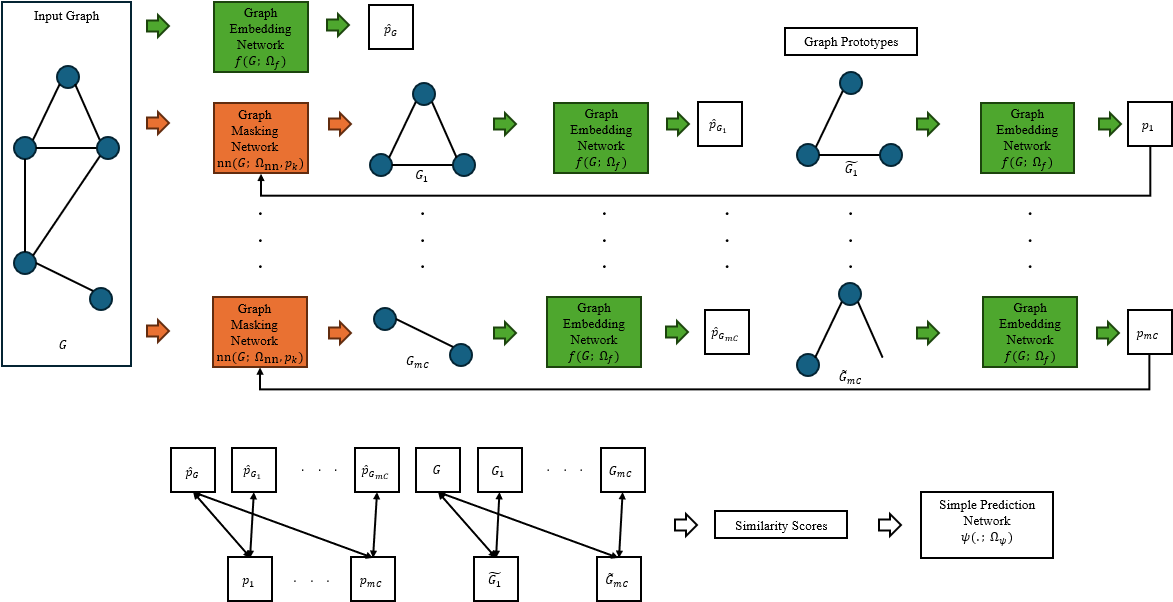
\includegraphics{figures/Graph_prot_diagram.png}

}

\caption{\label{fig-graph-prot_diag}Potential GNN based architecture
using graph protoypes.}

\end{figure}

\pagebreak

\hypertarget{references}{%
\section{References}\label{references}}

\hypertarget{refs}{}
\begin{CSLReferences}{1}{0}
\leavevmode\vadjust pre{\hypertarget{ref-bai2019unsupervised}{}}%
Bai, Yunsheng, Hao Ding, Yang Qiao, Agustin Marinovic, Ken Gu, Ting
Chen, Yizhou Sun, and Wei Wang. 2019. {``Unsupervised Inductive
Graph-Level Representation Learning via Graph-Graph Proximity.''}
\url{https://arxiv.org/abs/1904.01098}.

\leavevmode\vadjust pre{\hypertarget{ref-Bougleux_Brun_Carletti_Foggia_Gauxfczuxe8re_Vento_2015}{}}%
Bougleux, Sébastien, Luc Brun, Vincenzo Carletti, Pasquale Foggia,
Benoit Gaüzère, and Mario Vento. 2015. {``A Quadratic Assignment
Formulation of the Graph Edit Distance,''} no. arXiv:1512.07494
(December). \url{http://arxiv.org/abs/1512.07494}.

\leavevmode\vadjust pre{\hypertarget{ref-Breiman_2001}{}}%
Breiman, Leo. 2001. {``Random Forests.''} \emph{Machine Learning} 45
(1): 5--32. \url{https://doi.org/10.1023/A:1010933404324}.

\leavevmode\vadjust pre{\hypertarget{ref-Chen_Wu_Gupta_Ying_2023}{}}%
Chen, Jialin, Shirley Wu, Abhijit Gupta, and Rex Ying. 2023.
{``D4Explainer: In-Distribution GNN Explanations via Discrete Denoising
Diffusion,''} no. arXiv:2310.19321 (October).
\url{https://doi.org/10.48550/arXiv.2310.19321}.

\leavevmode\vadjust pre{\hypertarget{ref-Cho_Lee_Lee_2010}{}}%
Cho, Minsu, Jungmin Lee, and Kyoung Mu Lee. 2010. {``Reweighted Random
Walks for Graph Matching.''} In \emph{Computer Vision -- ECCV 2010},
edited by Kostas Daniilidis, Petros Maragos, and Nikos Paragios,
492--505. Lecture Notes in Computer Science. Berlin, Heidelberg:
Springer. \url{https://doi.org/10.1007/978-3-642-15555-0_36}.

\leavevmode\vadjust pre{\hypertarget{ref-Coulom2006EfficientSA}{}}%
Coulom, Rémi. 2006. {``Efficient Selectivity and Backup Operators in
Monte-Carlo Tree Search.''} In \emph{Computers and Games}.
\url{https://api.semanticscholar.org/CorpusID:16724115}.

\leavevmode\vadjust pre{\hypertarget{ref-Debnath_1991}{}}%
Debnath, Asim Kumar, Rosa L. Lopez de Compadre, Gargi Debnath, Alan J.
Shusterman, and Corwin Hansch. 1991. {``Structure-Activity Relationship
of Mutagenic Aromatic and Heteroaromatic Nitro Compounds. Correlation
with Molecular Orbital Energies and Hydrophobicity.''} \emph{Journal of
Medicinal Chemistry} 34 (2): 786--97.
\url{https://doi.org/10.1021/jm00106a046}.

\leavevmode\vadjust pre{\hypertarget{ref-erdds1959random}{}}%
ERDdS, P, and A R\&wi. 1959. {``On Random Graphs i.''} \emph{Publ. Math.
Debrecen} 6 (290-297): 18.

\leavevmode\vadjust pre{\hypertarget{ref-gallicchio2019fast}{}}%
Gallicchio, Claudio, and Alessio Micheli. 2019. {``Fast and Deep Graph
Neural Networks.''} \url{https://arxiv.org/abs/1911.08941}.

\leavevmode\vadjust pre{\hypertarget{ref-Gilbert_1959}{}}%
Gilbert, E. N. 1959. {``Random Graphs.''} \emph{The Annals of
Mathematical Statistics} 30 (4): 1141--44.

\leavevmode\vadjust pre{\hypertarget{ref-Gretton_Borgwardt_Rasch_Schuxf6lkopf_Smola_2012}{}}%
Gretton, Arthur, Karsten M. Borgwardt, Malte J. Rasch, Bernhard
Schölkopf, and Alexander Smola. 2012. {``A Kernel Two-Sample Test.''}
\emph{Journal of Machine Learning Research} 13 (25): 723--73.

\leavevmode\vadjust pre{\hypertarget{ref-Huijben_Kool_Paulus_van_Sloun_2022}{}}%
Huijben, Iris A. M., Wouter Kool, Max B. Paulus, and Ruud J. G. van
Sloun. 2022. {``A Review of the Gumbel-Max Trick and Its Extensions for
Discrete Stochasticity in Machine Learning,''} no. arXiv:2110.01515
(March). \url{https://doi.org/10.48550/arXiv.2110.01515}.

\leavevmode\vadjust pre{\hypertarget{ref-Maddison_Mnih_Teh_2017}{}}%
Maddison, Chris J., Andriy Mnih, and Yee Whye Teh. 2017. {``The Concrete
Distribution: A Continuous Relaxation of Discrete Random Variables,''}
no. arXiv:1611.00712 (March).
\url{https://doi.org/10.48550/arXiv.1611.00712}.

\leavevmode\vadjust pre{\hypertarget{ref-Maron_Ben-Hamu_Serviansky_Lipman_2020}{}}%
Maron, Haggai, Heli Ben-Hamu, Hadar Serviansky, and Yaron Lipman. 2020.
{``Provably Powerful Graph Networks,''} no. arXiv:1905.11136 (June).
\url{https://doi.org/10.48550/arXiv.1905.11136}.

\leavevmode\vadjust pre{\hypertarget{ref-olah2020zoom}{}}%
Olah, Chris, Nick Cammarata, Ludwig Schubert, Gabriel Goh, Michael
Petrov, and Shan Carter. 2020. {``Zoom in: An Introduction to
Circuits.''} \emph{Distill}.
\url{https://doi.org/10.23915/distill.00024.001}.

\leavevmode\vadjust pre{\hypertarget{ref-Rado1964UniversalGA}{}}%
Rado, Richard. 1964. {``Universal Graphs and Universal Functions.''}
\emph{Acta Arithmetica} 9: 331--40.
\url{https://api.semanticscholar.org/CorpusID:118279788}.

\leavevmode\vadjust pre{\hypertarget{ref-Rudin_2019}{}}%
Rudin, Cynthia. 2019. {``Stop Explaining Black Box Machine Learning
Models for High Stakes Decisions and Use Interpretable Models
Instead,''} no. arXiv:1811.10154 (September).
\url{https://doi.org/10.48550/arXiv.1811.10154}.

\leavevmode\vadjust pre{\hypertarget{ref-Steck_Ekanadham_Kallus_2024}{}}%
Steck, Harald, Chaitanya Ekanadham, and Nathan Kallus. 2024. {``Is
Cosine-Similarity of Embeddings Really about Similarity?''} March.
\url{https://doi.org/10.1145/3589335.3651526}.

\leavevmode\vadjust pre{\hypertarget{ref-Vignac_Krawczuk_Siraudin_Wang_Cevher_Frossard_2023}{}}%
Vignac, Clement, Igor Krawczuk, Antoine Siraudin, Bohan Wang, Volkan
Cevher, and Pascal Frossard. 2023. {``DiGress: Discrete Denoising
Diffusion for Graph Generation,''} no. arXiv:2209.14734 (May).
\url{https://doi.org/10.48550/arXiv.2209.14734}.

\leavevmode\vadjust pre{\hypertarget{ref-wang2024pygm}{}}%
Wang, Runzhong, Ziao Guo, Wenzheng Pan, Jiale Ma, Yikai Zhang, Nan Yang,
Qi Liu, et al. 2024. {``Pygmtools: A Python Graph Matching Toolkit.''}
\emph{Journal of Machine Learning Research} 25 (33): 1--7.
\url{https://jmlr.org/papers/v25/23-0572.html}.

\leavevmode\vadjust pre{\hypertarget{ref-Wang_Shen_2024}{}}%
Wang, Xiaoqi, and Han-Wei Shen. 2024. {``GNNInterpreter: A Probabilistic
Generative Model-Level Explanation for Graph Neural Networks,''} no.
arXiv:2209.07924 (February).
\url{https://doi.org/10.48550/arXiv.2209.07924}.

\leavevmode\vadjust pre{\hypertarget{ref-Xiao_Wang_Rong_Yang_Zhang_Zhan_Bishop_Wilhelm_Zhang_Pickering_et_al._2023}{}}%
Xiao, Guanghua, Shidan Wang, Ruichen Rong, Donghan Yang, Xinyi Zhang,
Xiaowei Zhan, Justin Bishop, et al. 2023. \emph{Deep Learning of Cell
Spatial Organizations Identifies Clinically Relevant Insights in Tissue
Images}. Preprint. In Review.
\url{https://doi.org/10.21203/rs.3.rs-2928838/v1}.

\leavevmode\vadjust pre{\hypertarget{ref-Yuan_Tang_Hu_Ji_2020}{}}%
Yuan, Hao, Jiliang Tang, Xia Hu, and Shuiwang Ji. 2020. {``XGNN: Towards
Model-Level Explanations of Graph Neural Networks.''} In
\emph{Proceedings of the 26th ACM SIGKDD International Conference on
Knowledge Discovery \& Data Mining}, 430--38.
\url{https://doi.org/10.1145/3394486.3403085}.

\leavevmode\vadjust pre{\hypertarget{ref-Yuan_Yu_Gui_Ji_2022}{}}%
Yuan, Hao, Haiyang Yu, Shurui Gui, and Shuiwang Ji. 2022.
{``Explainability in Graph Neural Networks: A Taxonomic Survey,''} no.
arXiv:2012.15445 (July).
\url{https://doi.org/10.48550/arXiv.2012.15445}.

\leavevmode\vadjust pre{\hypertarget{ref-Zhang_Liu_Wang_Lu_Lee_2021}{}}%
Zhang, Zaixi, Qi Liu, Hao Wang, Chengqiang Lu, and Cheekong Lee. 2021.
{``ProtGNN: Towards Self-Explaining Graph Neural Networks,''} no.
arXiv:2112.00911 (December).
\url{https://doi.org/10.48550/arXiv.2112.00911}.

\end{CSLReferences}



\end{document}
